\documentclass[11pt,a4paper]{article}

% ---------------------------------------------------------------------------
% Supervised Fine-Tuning of Small Vision-Language Models for Fully Automated
% Chest-Radiograph Reporting: Data, Model Development, and Training Methodology
% A Technical Report
% ---------------------------------------------------------------------------

\usepackage[utf8]{inputenc}
\usepackage[T1]{fontenc}
\usepackage{lmodern}
\usepackage[margin=1in]{geometry}
\usepackage{amsmath,amssymb}
\usepackage{graphicx}
\usepackage{booktabs}
\usepackage{longtable}
\usepackage{array}
\usepackage{tabularx}
\usepackage{multirow}
\usepackage{xcolor}
\usepackage{listings}
\usepackage{enumitem}
\usepackage{fancyhdr}
\usepackage{titlesec}
\usepackage{parskip}
\usepackage[hidelinks]{hyperref}
\usepackage{microtype}
\usepackage{caption}
\usepackage{float}

% ---- listing style for code / data snippets ----
\definecolor{codebg}{RGB}{247,248,250}
\definecolor{codekw}{RGB}{40,90,180}
\definecolor{codecm}{RGB}{110,120,135}
\lstset{
  basicstyle=\ttfamily\footnotesize,
  backgroundcolor=\color{codebg},
  frame=single,
  rulecolor=\color{codecm!30},
  breaklines=true,
  breakatwhitespace=false,
  columns=fullflexible,
  keepspaces=true,
  showstringspaces=false,
  keywordstyle=\color{codekw}\bfseries,
  commentstyle=\color{codecm}\itshape,
  xleftmargin=6pt,
  framexleftmargin=4pt,
}

\newcolumntype{R}{>{\raggedleft\arraybackslash}X}
\newcolumntype{L}{>{\raggedright\arraybackslash}X}

\pagestyle{fancy}
\fancyhf{}
\fancyhead[L]{\footnotesize VLM Autoreporting for Chest Radiographs}
\fancyhead[R]{\footnotesize\thepage}
\renewcommand{\headrulewidth}{0.4pt}

\linespread{1.06}
\titleformat{\section}{\normalfont\Large\bfseries}{\thesection}{0.6em}{}
\titleformat{\subsection}{\normalfont\large\bfseries}{\thesubsection}{0.6em}{}
\titleformat{\subsubsection}{\normalfont\normalsize\bfseries}{\thesubsubsection}{0.6em}{}

\title{\vspace{-1.5em}\textbf{Supervised Fine-Tuning of Small Vision--Language Models\\ for Fully Automated Chest-Radiograph Reporting:\\ Data, Model Development, and Training Methodology}\\[0.6em]
\large A Technical Report}
\author{}
\date{}

\begin{document}

\maketitle
\thispagestyle{fancy}

% ===========================================================================
\begin{abstract}
\noindent
We present the design, data engineering, model development, and supervised fine-tuning (SFT) methodology behind a family of small vision--language models (VLMs) built for \emph{fully automated} chest-radiograph (chest X-ray, CXR) reporting. Rather than treating report generation as a single free-text captioning task, we decompose the clinical act of reading a chest radiograph into a chain of explicit, machine-checkable sub-tasks: (i) \emph{pathology classification} over a controlled vocabulary of 132 special abnormality/device tokens; (ii) \emph{spatial grounding} via bounding-box prediction and box$\leftrightarrow$label matching; (iii) \emph{symbolic reasoning} expressed in an Answer-Set-Programming (ASP)-style scene graph with multi-level, step-wise diagnostic analysis; (iv) \emph{structured ontology reporting} comprising Findings, Summary, Complete Reasoning, Impression, Recommendations, and a Prominence Score; (v) \emph{hierarchical positive-findings graphs} and finding triples; and (vi) \emph{multi-image report comparison} for longitudinal and multi-view studies. The training corpus spans roughly 6.16 million supervised conversations drawn from public datasets (MIMIC-CXR, CheXpert), a licensed commercial source (Segmed), and a large proprietary internal cohort, with a subset of synthetic examples. We describe the full data-preparation pipeline --- schema unification, per-record image/\texttt{<image>}-token validation over 100\% of records, source-stratified length and prevalence analysis, empty-response detection, partial-write corruption detection, and a lazy, on-the-fly medical-image augmentation path adapted from a 2-D vision foundation pipeline. On the modeling side we compare two backbone families --- InternVL3.5 (2B/8B, InternViT-300M + Qwen3 language model) and Qwen3.5 (2B/4B, a hybrid-thinking model built on GatedDeltaNet) --- and document how architectural differences dictate which throughput optimizations (sequence packing, padding-free collation) are available. We detail the SFT recipe end-to-end within the ms-swift framework: full-parameter fine-tuning of the vision encoder, MLP aligner, and language model; vocabulary extension with 132 new special tokens; a non-thinking-prefix scheme with an \texttt{ignore\_empty\_think} loss mask; Liger-kernel fused operators; DeepSpeed ZeRO-2/ZeRO-3; and three complementary data-loading strategies (in-memory tokenization, pre-tokenized cached datasets with train-time packing, and lazy tokenization for stochastic augmentation). We report training dynamics (final train loss 0.371, eval loss 0.361, token accuracy 0.874 for the InternVL3.5-2B run over 12{,}571 optimizer steps) and a held-out evaluation on a curated 25{,}487-study high-confidence (``easy'') subset drawn from a 136{,}639-study valid-ground-truth pool (itself distilled from 145{,}735 studies after quarantining 6.07\% corrupt inputs), including image-integrity auditing, predicted-token distribution, per-tag and per-parent-class sensitivity/specificity/precision, and a focused nodule false-negative error analysis. On the 25k subset the model reaches a per-tag macro sensitivity of 0.874 and a 25-parent-class macro of 0.863 sensitivity / 0.863 specificity, with devices and major pathologies performing strongest. We close with a candid discussion of failure modes and outline the path from SFT to preference optimization and reinforcement learning. This report is written as a reproducible engineering record: every dataset, hyperparameter, and analysis script referenced here is enumerated in the appendices.
\end{abstract}

\tableofcontents
\newpage

% ===========================================================================
\section{Introduction}

\subsection{Motivation}
Chest radiography is the highest-volume diagnostic imaging examination in the world. A single large hospital network can acquire tens of thousands of chest radiographs per day, and in many parts of the world the ratio of radiologists to studies is such that a large fraction of images are never formally read, or are read only after a delay that erodes their clinical value. The economic and clinical case for \emph{automated preliminary reporting} --- a system that reads an image and produces a structured, human-readable, clinically-actionable draft report --- is therefore compelling. Such a system does not replace the radiologist; it triages, pre-populates, and standardizes, so that the scarce human expert spends their attention where it matters most.

The last three years have made this ambition technically plausible. General-purpose vision--language models (VLMs) --- models that fuse a vision encoder with a large language model (LLM) through a lightweight projector --- have reached a level of visual grounding and language fluency where, with domain adaptation, they can describe medical images in clinically meaningful terms. The open-source ecosystem now ships strong small VLMs (2--8B parameters) that are cheap enough to fine-tune fully and to serve at scale, and mature training frameworks (ms-swift, and kernels such as Liger and Flash-Attention) that make multi-million-example supervised fine-tuning practical on a single 8-GPU node.

This report documents the end-to-end construction of such a system: a \emph{full-autoreporting} VLM for chest radiographs. The emphasis throughout is on \textbf{data preparation and training methodology}, because in our experience these --- far more than the choice of backbone --- determine whether the resulting model is clinically usable. We treat the report not as an opaque string to be produced by a black box, but as the terminal node of an explicit reasoning chain that the model is trained to externalize: classify, localize, reason symbolically, and only then write the structured report. This decomposition is the organizing principle of both the data and the model.

\subsection{What ``full autoreporting'' means here}
A radiologist reading a chest film does several things almost simultaneously: they recognize abnormalities and devices, they localize them, they reason about severity and differential diagnosis in light of the clinical context, and they compose a report with a conventional structure (Findings $\rightarrow$ Impression $\rightarrow$ Recommendations). A model that only emits free-text prose short-circuits all of the intermediate structure, which makes it (a) hard to verify, (b) hard to integrate with downstream clinical software, and (c) prone to fluent-but-wrong ``hallucinated'' findings.

Our design instead makes each intermediate representation an \emph{explicit, supervised output}:
\begin{itemize}[leftmargin=1.4em]
  \item \textbf{Classification} produces a set of controlled special tokens (e.g.\ \texttt{<ATELECTASIS>}, \texttt{<PLEURAL\_EFFUSION>}, \texttt{<ENDOTRACHEAL\_TUBE>}) --- a machine-readable label set that can be scored directly against structured ground truth.
  \item \textbf{Grounding} produces bounding boxes for findings and devices, and separately matches boxes to labels, giving spatial accountability.
  \item \textbf{Symbolic reasoning} produces an Answer-Set-Programming-style scene graph (\texttt{finding(...)}, \texttt{location(...)}, \texttt{severity(...)}, \texttt{characteristic(...)}) followed by step-wise diagnostic analysis --- a transparent, inspectable reasoning trace.
  \item \textbf{Structured reporting} produces a fixed-schema ontology report: Findings, Summary, Complete Reasoning, Impression, Recommendations, and a numeric Prominence Score.
  \item \textbf{Hierarchical graphs and triples} encode the positive findings as a graph, giving a compact knowledge-graph view of a study.
  \item \textbf{Comparison} ingests two or more images and produces a structured comparison --- the substrate for longitudinal follow-up and multi-view reasoning.
\end{itemize}

Crucially, these are \emph{composed} in training data: some examples ask for one sub-task in isolation, some chain all of them into a single long reply, and some split them across multiple conversational turns. The model therefore learns both the individual skills and the full pipeline, and at inference time we can ask it for exactly as much structure as the downstream consumer needs.

\subsection{Contributions}
This report contributes:
\begin{enumerate}[leftmargin=1.6em]
  \item A reproducible data-engineering methodology for assembling a $\sim$6.16M-conversation multi-task CXR corpus from heterogeneous sources, including a 100\%-coverage structural validation invariant (image count $=$ \texttt{<image>}-token count), source-stratified statistical characterization, and systematic data-quality auditing.
  \item A task decomposition that turns report generation into a chain of machine-checkable sub-tasks, realized as a controlled vocabulary of 132 abnormality/device tokens plus ASP-style symbolic reasoning and a fixed-schema ontology report.
  \item A detailed, comparative SFT methodology across two backbone families that documents how backbone architecture governs the availability of throughput optimizations, and that lays out three interoperable data-loading strategies.
  \item A large-scale evaluation and error analysis over 145{,}735 held-out studies, including an image-integrity audit that identified and quarantined 6.07\% corrupt inputs.
  \item A candid account of failure modes and their causes, distinguishing genuine model limitations from artifacts of exact-match scoring against a free-form 18k-name ground-truth vocabulary.
\end{enumerate}

\subsection{Document structure}
Sections~\ref{sec:data-sources}--\ref{sec:augment} constitute the data half of the report and are deliberately the longest, reflecting where most of the engineering effort --- and most of the eventual model quality --- resides. Sections~\ref{sec:backbone}--\ref{sec:deploy} cover model development, the SFT recipe, and the systems engineering that made multi-million-example training tractable. Sections~\ref{sec:eval-protocol}--\ref{sec:nodule} present the evaluation and error analysis. Sections~\ref{sec:discussion}--\ref{sec:conclusion} discuss, bound, and project the work forward. The appendices enumerate every dataset, the full 132-token vocabulary, all hyperparameters, and the analysis scripts.

% ===========================================================================
\section{Preliminaries and Notation}
\label{sec:prelim}

For self-containedness we fix terminology and notation used throughout; the glossary (Appendix~\ref{app:glossary}) gives fuller definitions.

\textbf{The model.} A VLM $f_\theta$ maps an instruction $q$ and a set of images $\{I_1,\dots,I_n\}$ to a text response $y$. Internally, each image is encoded by a ViT into visual tokens, projected by the aligner into the LLM embedding space, spliced into the token stream at the positions of the \texttt{<image>} placeholders in $q$, and decoded autoregressively: $y \sim p_\theta(\cdot \mid q, I_{1:n})$.

\textbf{The label alphabet.} $\mathcal{V}$ denotes the controlled 132-token finding vocabulary (Appendix~\ref{app:vocab}). The classification output of a study is a subset $S \subseteq \mathcal{V}$ --- the tokens the model emits in its header. A finding token $\langle X\rangle$ is \emph{predicted-positive} for a study iff $\langle X\rangle \in S$.

\textbf{Ground truth.} A study's ground truth is a set $G$ of free-form finding names (with \texttt{presence=true}). A mapping $\phi: (\text{GT names}) \to \mathcal{V}\cup\{\varnothing\}$ associates GT names with controlled tokens; a token $\langle X\rangle$ is \emph{GT-positive} iff some $g\in G$ has $\phi(g)=\langle X\rangle$. Parent classes group tokens into clinical super-categories (Section~\ref{sec:taxonomy}).

\textbf{Metrics.} For a fixed token/parent, over the evaluation population: $\mathrm{TP}$ (predicted-$+$, GT-$+$), $\mathrm{FP}$ (predicted-$+$, GT-$-$), $\mathrm{FN}$ (predicted-$-$, GT-$+$), $\mathrm{TN}$ (predicted-$-$, GT-$-$); $\text{sensitivity}=\mathrm{TP}/(\mathrm{TP}{+}\mathrm{FN})$, $\text{specificity}=\mathrm{TN}/(\mathrm{TN}{+}\mathrm{FP})$, $\text{precision}=\mathrm{TP}/(\mathrm{TP}{+}\mathrm{FP})$. \emph{Macro} averages take the unweighted mean over classes.

\textbf{Data conventions.} A \emph{conversation} is one (images, turns) record; a \emph{task family} is a JSONL file rendering a pool of studies into one instruction type; \emph{provenance} is the source class (chexpert/mimic/segmed/internal/synthetic/prod) inferred from the image path.

% ===========================================================================
\section{Background and Related Work}

\subsection{Vision--language models and the ViT--MLP--LLM paradigm}
Modern open VLMs overwhelmingly adopt a three-part architecture: a \textbf{vision encoder} (typically a Vision Transformer, ViT) that maps an image to a grid of visual tokens; a lightweight \textbf{projector / aligner} (usually a two-layer MLP) that maps visual-token embeddings into the language model's embedding space; and a \textbf{large language model} that consumes the projected visual tokens interleaved with text tokens and generates text autoregressively. This ``ViT--MLP--LLM'' recipe is the backbone of the LLaVA line of work and of the InternVL family, and it is the paradigm of both of our chosen backbones.

Two architectural details matter for medical imaging. First, \textbf{dynamic high resolution}: because diagnostic findings on a chest radiograph can be small (a sub-centimeter nodule, a thin pneumothorax line, the tip of a catheter), the vision encoder must ingest the image at a resolution high enough to preserve those features. InternVL's dynamic-high-resolution tiling --- splitting a large image into multiple fixed-size tiles, each encoded independently --- retains fine detail while keeping per-tile compute bounded. Second, \textbf{visual-token compression}: InternVL3.5 encodes each tile to on the order of 1{,}024 visual tokens and then compresses them (via a pixel-shuffle operation) to 256 tokens before the LLM, trading a controlled amount of spatial resolution for a 4$\times$ reduction in sequence length. Our training controls the visual-token budget explicitly through the \texttt{IMAGE\_MAX\_TOKEN\_NUM} / \texttt{INPUT\_SIZE} knobs (Section~\ref{sec:sft}).

\subsection{Automated chest-radiograph report generation}
Automated CXR interpretation and report generation is an active field, and three generations of approaches can be distinguished. Early work used CNN encoders with RNN/transformer decoders trained end-to-end on MIMIC-CXR to produce free-text findings. A second generation built \emph{foundation models} specifically for chest imaging: \textbf{CheXagent} (Stanford AIMI) couples a clinical LLM for parsing reports, a CXR vision encoder, and a bridging network, and is evaluated on the multi-task CheXbench suite. A third generation adds \textbf{grounding and structure}: \textbf{MAIRA-2} (a 7B radiology VLM trained on MIMIC-CXR, PadChest, and a US multi-site mix) performs \emph{grounded} report generation --- producing not only clinically accurate text but also the spatial locations of the findings it describes --- and is evaluated with a sentence-level correctness/completeness framework (RadFact) that uses an LLM as judge. A parallel line of ``agentic'' systems (MedRAX, CXR-Agent) orchestrates multiple tools and reasoning stages with uncertainty-aware reporting.

Our work sits in the third generation but differs in emphasis. Where MAIRA-2 grounds \emph{phrases} in a free-text report, we make the \emph{entire intermediate representation} explicit and supervised --- a controlled classification vocabulary, an ASP-style symbolic scene graph, and a fixed-schema ontology report --- so that the report is the endpoint of an inspectable chain rather than a single generative leap. This is a deliberate bet: structure buys verifiability and downstream integrability at the cost of requiring far more elaborate training data, which is precisely why the data-engineering sections of this report are so extensive. Table~\ref{tab:related} situates our system among representative CXR reporting models along the axes that matter for our design.

\begin{table}[H]
\centering\footnotesize
\caption{Representative chest-radiograph reporting systems and where this work differs. ``Controlled vocab.'' $=$ a closed label set for the scored output; ``Symbolic reasoning'' $=$ an explicit machine-parseable reasoning trace.}
\label{tab:related}
\begin{tabularx}{\textwidth}{L c c c c}
\toprule
\textbf{System} & \textbf{Backbone size} & \textbf{Grounding} & \textbf{Controlled vocab.} & \textbf{Symbolic reasoning} \\
\midrule
CheXagent & $\sim$8B & no & partial (CheXbench tasks) & no \\
MAIRA-2 & $\sim$7B & yes (phrase boxes) & no (free text) & no \\
MedRAX / CXR-Agent & agentic (tool LLM) & via tools & no & partial (tool traces) \\
\textbf{This work} & \textbf{2--8B} & \textbf{yes (boxes $+$ match)} & \textbf{yes (132 tokens)} & \textbf{yes (ASP scene graph)} \\
\bottomrule
\end{tabularx}
\end{table}

\subsection{Structured and neuro-symbolic reasoning}
Free-text chain-of-thought is difficult to verify. Answer Set Programming (ASP) is a declarative logic-programming formalism in which a problem is specified as a set of logical facts and rules and solved by finding \emph{stable models} (answer sets). We do not run an ASP solver at inference time; instead we borrow ASP's \emph{representational discipline}. Each study's reasoning trace begins with a symbolic scene graph written in ASP-like syntax --- \texttt{finding(cardiac\_silhouette).}, \texttt{location(cardiac\_silhouette, mediastinum).}, \texttt{severity(cardiac\_silhouette, normal).} --- followed by multi-level, step-wise diagnostic analysis in natural language. The value of this format is that it forces the model to \emph{name} each finding, its location, its severity, and its characteristics as discrete, parseable predicates before it commits to prose. This is a lightweight form of neuro-symbolic modeling: the neural model emits symbolic structure that is both a scaffold for its own reasoning and an artifact that downstream software (or a human reviewer) can inspect.

\subsection{Efficient supervised fine-tuning: kernels, packing, and frameworks}
Full-parameter SFT of a VLM on millions of long, multimodal examples is compute- and memory-bound, and three now-standard techniques make it tractable on a single node.

\textbf{Fused kernels (Liger).} Liger Kernel is a collection of Triton kernels for LLM training that fuse micro-pipeline patterns --- RMSNorm, RoPE, SwiGLU, and especially a fused linear~$+$~cross-entropy that avoids materializing the full logits tensor --- into register-resident operations that minimize high-bandwidth-memory traffic. In published benchmarks Liger increases multi-GPU training throughput by roughly 20\% and cuts memory use by up to 60\% relative to stock HuggingFace implementations, and it composes cleanly with Flash-Attention, FSDP, and DeepSpeed. We enable Liger (\texttt{--use\_liger\_kernel true}) in every training run; the memory headroom it frees is what lets us push per-device batch sizes and the 28k-token context window.

\textbf{Sequence packing and padding-free collation.} In a naïvely batched dataset, short sequences are padded to the length of the longest sequence in the batch, and the padding tokens waste compute. \emph{Packing} concatenates multiple variable-length examples into one long sequence up to the context window, storing sequence boundaries so that attention can be restricted within each original example. With a Flash-Attention backend, the boundaries are passed as cumulative sequence lengths (\texttt{cu\_seqlens}), which lets the kernel compute attention per-segment without a quadratic mask and without cross-contamination between packed examples. Packing raises the fraction of \emph{meaningful} tokens per batch dramatically --- reported utilization improvements from $\sim$10\% to $\sim$98\% in the extreme --- for a 1.1--2$\times$ wall-clock speedup and $\sim$30\% memory reduction, with no loss in quality. \emph{Padding-free} is the collation-time cousin: it removes padding at the collator without pre-encoding the whole dataset.

\textbf{Training framework (ms-swift).} We build on ms-swift (the ModelScope Swift toolkit), which provides a unified \texttt{swift sft} / \texttt{swift export} / \texttt{swift infer} / \texttt{swift deploy} CLI over a very large model zoo, with first-class support for multimodal templates, full and parameter-efficient tuning, DeepSpeed, Liger, packing/padding-free, cached (pre-tokenized) datasets, and multiple inference backends (vLLM, SGLang, LMDeploy). ms-swift's \emph{template} abstraction --- which knows how to interleave \texttt{<image>} placeholders, apply the chat format, and mask the loss over designated spans --- is the layer into which we inject our medical-image augmentation and path-resolution logic (Section~\ref{sec:infra}).

\subsection{Datasets in the public CXR ecosystem}
Our corpus draws on the two canonical public chest-radiograph datasets and augments them with licensed and internal data. \textbf{MIMIC-CXR} is a large, de-identified dataset of chest radiographs with free-text reports from the Beth Israel Deaconess Medical Center. \textbf{CheXpert} is a large labeled CXR dataset from Stanford with uncertainty-aware labels for 14 observations. To these we add \textbf{Segmed}, a commercial provider of de-identified, consented multi-site medical imaging data (which contributes the plurality of our multi-source examples), a large \textbf{internal} proprietary cohort, and a small quantity of \textbf{synthetic} examples.

% ===========================================================================
\section{System Overview and Task Formulation}

\subsection{The inference-time contract}
At inference, the system is a single VLM served behind an OpenAI-compatible endpoint (Section~\ref{sec:deploy}). It accepts one or more chest-radiograph images and a natural-language instruction, and returns text. The \emph{instruction} selects which of the trained sub-tasks the model performs. Because the training data pairs each sub-task with a stable instruction template (Section~\ref{sec:schema}), the downstream caller has a menu of well-defined behaviors --- from a bare classification token set (cheap, fast, directly scoreable) to the full ontology report. The individual pieces of the ontology report are \emph{also} independently addressable, because the training corpus contains those single-turn variants.

\subsection{The response format}
Every trained response uses a consistent internal structure that mirrors the reasoning chain. A response to the full pipeline begins with an (empty) \texttt{<think>} block --- the \emph{non-thinking} marker required by the hybrid-thinking Qwen3.5 backbone (Section~\ref{sec:sft}) --- followed by the predicted classification tokens emitted between \texttt{</think>} and a delimited \texttt{<|ASP>|}\,\dots\,\texttt{<|/ASP>|} reasoning section, and finally the structured ontology report. The classification tokens up front are not decoration: they are the machine-readable label set that our evaluation scores directly (Section~\ref{sec:eval-protocol}), and they act as a \emph{plan} that conditions the subsequent reasoning and report.

\subsection{Why decomposition, concretely}
Consider a study with a subtle right-apical pneumothorax and an endotracheal tube. A free-text-only model must get everything right in one generative pass, and if it omits the pneumothorax there is no intermediate signal that anything was missed. Under our decomposition, the failure is \emph{localized and observable}: either \texttt{<PNEUMOTHORAX>} is absent from the classification header (a classification error we can measure against structured GT), or it is present in the header but dropped from the report (a report-consistency error), or the bounding-box task fails to localize it (a grounding error). Each of these is separately trainable and separately measurable. The evaluation in Sections~\ref{sec:eval-protocol}--\ref{sec:nodule} is only possible \emph{because} of this decomposition.

\subsection{Scope of this report}
This report covers the supervised fine-tuning stage. It documents multiple training runs --- InternVL3.5-2B and 8B, and Qwen3.5-2B and 4B --- that share a data corpus and a recipe but differ in backbone and in which throughput optimizations are enabled. The flagship analyzed model is a Qwen3.5-2B checkpoint (\texttt{checkpoint-5191}) evaluated on 145{,}735 studies, complemented by an InternVL3.5-2B run whose full training curves we present. Preference optimization (DPO/MPO) and reinforcement learning (GRPO) are out of scope and are discussed only as future work (Section~\ref{sec:future}).

% ===========================================================================
\section{Data: Sources and Provenance}
\label{sec:data-sources}

\subsection{Overview}
The training corpus is a \textbf{deduplicated union of nine large JSONL files} totaling \textbf{6{,}160{,}387 supervised conversations}. Each file is a \emph{task family} (Section~\ref{sec:schema}): the same underlying pool of chest radiographs is rendered into different instruction/response pairs. Because one study can appear in several task families, the 6.16M \emph{conversations} correspond to a substantially smaller number of \emph{unique images} --- the multiplicity is intentional and is what teaches the model the full menu of behaviors. Table~\ref{tab:files} lists the nine files, their row counts, and their roles.

\begin{table}[H]
\centering\footnotesize
\caption{The nine task-family files comprising the training corpus.}
\label{tab:files}
\begin{tabularx}{\textwidth}{L r c L}
\toprule
\textbf{File (task family)} & \textbf{Rows} & \textbf{Turns} & \textbf{Role} \\
\midrule
\texttt{bbox\_comparison\_550k} & 562{,}619 & 2 & Multi-image finding comparison (2--3 images) \\
\texttt{bbox\_label\_matching\_617k} & 617{,}858 & 2 & Box$\leftrightarrow$label matching (coords in prompt) \\
\texttt{cls\_token\_mimic\_chex\_segmed} & 637{,}941 & 2 & Classification (controlled token set) \\
\texttt{combined\_cls\_asp\_report} & 455{,}382 & 2 & Full pipeline in a single reply \\
\texttt{multiturn\_cls\_asp\_report} & 455{,}382 & 6 & Same pipeline split across 3 turns \\
\texttt{prod\_cls\_token} & 852{,}340 & 2 & Production classification (deploy dist.) \\
\texttt{hierarchical\_graph} & 1{,}451{,}706 & 2 & Hierarchical graph $+$ finding triples \\
\texttt{report\_comparison\_deepseek\_490k} & 490{,}796 & 2 & Report comparison (DeepSeek-generated) \\
\texttt{full\_tag\_extraction} & 636{,}363 & 2 & Structured JSON tag extraction \\
\midrule
\textbf{Total} & \textbf{6{,}160{,}387} & & \\
\bottomrule
\end{tabularx}
\end{table}

The \texttt{combined\_cls\_asp\_report} and \texttt{multiturn\_cls\_asp\_report} files have \emph{identical} row counts (455{,}382) because they are the same source samples rendered two ways: the \emph{combined} form puts all three tasks (classify $\rightarrow$ ASP-reason $\rightarrow$ ontology report) in one assistant turn (2 messages), while the \emph{multiturn} form splits the same content across three user/assistant exchanges (6 messages). Training on both teaches the model to produce the pipeline either as one monolithic response or interactively.

\subsection{Image sources}
Each conversation's images resolve to one of six provenance classes, inferred deterministically from the image path:
\begin{itemize}[leftmargin=1.4em]
  \item \textbf{\texttt{chexpert}} --- Stanford CheXpert studies.
  \item \textbf{\texttt{mimic}} --- MIMIC-CXR studies (Beth Israel).
  \item \textbf{\texttt{segmed}} --- licensed, consented, de-identified multi-site data from Segmed; the largest contributor to the multi-source families ($\sim$45--55\% of rows).
  \item \textbf{\texttt{internal}} --- a large proprietary internal cohort; dominant in the grounding/comparison families (85--88\% of the bbox families).
  \item \textbf{\texttt{synthetic}} --- a small quantity of synthetic images ($\sim$10--14\% of the bbox families), used to enrich the bounding-box coordinate distribution.
  \item \textbf{\texttt{prod}} --- the production distribution (852{,}340 classification rows), representing the true deployment image mix.
\end{itemize}
The source mix is \textbf{stable across the mimic/chex/segmed task families} ($\sim$24\% chexpert, $\sim$31\% mimic, $\sim$45\% segmed) because those families are drawn from the same study pool and differ only in how each study is rendered into a task. Section~\ref{sec:stats} shows systematic differences in output length and finding prevalence by source (chexpert studies carry more findings per study and produce the longest outputs; segmed carries the most ``no-abnormality'' studies).

\subsection{Ground-truth generation and teacher models}
The supervised targets were generated by a mixture of human-derived labels and strong teacher LLMs applied to source reports and structured findings. \textbf{Classification tokens} derive from structured finding labels mapped onto the controlled 132-token vocabulary (Section~\ref{sec:vocab}). \textbf{The ASP reasoning and ontology reports} were synthesized by prompting strong LLMs (Gemini-class models for the segmed/chexpert/mimic report families --- cf.\ the \texttt{\_gemini\_response} file naming --- and DeepSeek for the report-comparison family --- cf.\ \texttt{\_deepseek\_490k}) with the study's findings and the target schema, so that each target is a well-structured instance of the desired output. \textbf{Bounding boxes} derive from the internal detection pipeline (and synthetic augmentation) at a known target resolution (the \texttt{1000res} / \texttt{target\_res} naming records the coordinate reference frame; Section~\ref{sec:grounding}).

This teacher-distillation approach is standard for bootstrapping structured behaviors that no public dataset supplies directly (there is no public dataset of ASP scene graphs for chest radiographs). Its principal risk --- that the student inherits the teacher's errors and stylistic tics --- is real and is discussed in Section~\ref{sec:discussion}. The mitigations applied at data-prep time were: (a)~using the \emph{original} structured findings, not the teacher's free text, as the source of the classification labels we actually score; (b)~validating every record structurally (Section~\ref{sec:validation}); and (c)~auditing for and quarantining the teacher's failure modes (empty responses, API-error strings).

\subsection{Two data directories and the deduplicated union}
The corpus was assembled from two staging directories that overlap. The reconciliation rules were:
\begin{enumerate}[leftmargin=1.6em]
  \item The dataset common to both directories --- \texttt{bbox\_comparison\_550k} (562{,}619 rows, byte-identical and clean in both) --- is included \textbf{once}.
  \item Where a file exists in a broken and a corrected version, the \textbf{corrected} version is used. Specifically, \texttt{08\_June\_2026\_final\_report\_comparison\_deepseek\_490k} was found to be \textbf{100\% broken} and was replaced by \texttt{23\_June\_2026\_corrected\_final\_report\_comparison\_deepseek\_490k}.
  \item \texttt{1\_Aug\_final\_data\_for\_pretraining\_cleaned} was \textbf{intentionally excluded} from the final production runs.
\end{enumerate}
The care taken here is not incidental: an earlier training run crashed because a regenerable dataset cache filled the shared root disk, and a report-comparison file that looked valid was in fact entirely broken. Both incidents motivated the validation regime of Section~\ref{sec:validation} and the disk-hygiene practices of Section~\ref{sec:infra}.

% ===========================================================================
\section{Data: Schema, Unification, and the Task Families}
\label{sec:schema}

\subsection{The unified record schema}
Records come in two structural variants; the training template handles both identically.

\textbf{Variant A --- single image.} A top-level \texttt{image} string and a \texttt{messages} list:
\begin{lstlisting}
{
  "image": "/localstorage/cxr_data/.../view1_frontal.png",
  "messages": [
    {"from": "human", "value": "Classify the abnormalities from the given chest xray.\n<image>"},
    {"from": "gpt",   "value": "<SURGICAL_HARDWARE> <CONSOLIDATION> ..."}
  ]
}
\end{lstlisting}

\textbf{Variant B --- multiple images.} A top-level \texttt{images} list and a \texttt{conversations} list:
\begin{lstlisting}
{
  "images": ["/path/img1.png", "/path/img2.png"],
  "conversations": [
    {"from": "human", "value": "... <image> ... <image> ..."},
    {"from": "gpt",   "value": "..."}
  ]
}
\end{lstlisting}

The invariants across both variants: the \textbf{image field} is \texttt{image} (single) or \texttt{images} (list); the \textbf{conversation field} is \texttt{messages} or \texttt{conversations}; each \textbf{turn} is \texttt{\{"from": "human"|"gpt", "value": "..."\}}; and the \textbf{\texttt{<image>} placeholder} appears inline in the human turn(s), exactly once per image, marking where the projected visual tokens are spliced into the token stream. The single most important structural invariant --- verified over 100\% of records (Section~\ref{sec:validation}) --- is:
\begin{quote}
\emph{The number of images in a record equals the number of \texttt{<image>} tokens in its conversation.}
\end{quote}
A mismatch here is catastrophic: the template would splice visual tokens into the wrong position or drop an image entirely, silently corrupting every example that survives.

\subsection{Task family 1 --- Classification (controlled token set)}
\textbf{Instruction (fixed):} ``Classify the abnormalities from the given chest xray.'' \textbf{Response:} a whitespace-separated sequence of controlled special tokens, e.g.\ \texttt{<SURGICAL\_HARDWARE> <CONSOLIDATION> <CARDIOMEGALY>}. This is the single most frequent prompt in the corpus: combining the plain, production, and pipeline classification families, ``Classify the abnormalities\dots'' accounts for \textbf{32.0\%} of all prompts (3{,}401{,}451 occurrences). The response is short (median $\sim$55 characters for the plain family; $\sim$462 for the richer production family), and the label set is drawn from the 132-token vocabulary of Appendix~\ref{app:vocab}. A non-trivial fraction of classification targets are legitimately \textbf{empty} --- a genuinely normal study has no abnormality tokens. In the plain family, 1{,}744 of 637{,}941 rows (0.27\%) have an empty response; these concentrate in the segmed source (1{,}007), consistent with segmed carrying more no-abnormality studies (Section~\ref{sec:validation}).

\subsection{Task family 2 --- Structured JSON tag extraction}
\textbf{Instruction (fixed):} ``Classify the abnormalities in the given chest x-ray in JSON format with presence, size, location and very short characterization.'' \textbf{Response:} a JSON object enumerating each finding with \texttt{presence}, \texttt{size}, \texttt{location}, and a short \texttt{characterization} (median $\sim$530 characters, up to $\sim$5{,}500). It is the format most directly comparable to the structured ground truth used in evaluation, whose GT ontology is itself a nested \texttt{finding} $\rightarrow$ \texttt{\{presence, size, location, characteristics\}} structure (Section~\ref{sec:eval-protocol}).

\subsection{Task family 3 --- ASP-style symbolic reasoning}
\textbf{Instruction:} e.g.\ ``Generate Answer Set Programming (ASP)-based reasoning for the provided medical image. Include multi-level diagnostic analysis and structured, step-wise clinical reasoning.'' \textbf{Response:} a delimited \texttt{<|ASP>|} section that opens with a first-person framing, then a \textbf{symbolic scene graph in ASP syntax}, then multi-level step-wise analysis. An abridged real target:
\begin{lstlisting}
<|ASP|>I am directly viewing the chest X-ray of this 52-year-old male, evaluating for any cardiopulmonary abnormalities...

STEP 1: SYMBOLIC SCENE GRAPH REPRESENTATION (ASP Format)
% ---- Findings ----
finding(cardiac_silhouette).
location(cardiac_silhouette, mediastinum).
severity(cardiac_silhouette, normal).
characteristic(cardiac_silhouette, normal_size_and_configuration).

finding(lung_parenchyma).
location(lung_parenchyma, bilateral).
severity(lung_parenchyma, normal).
characteristic(lung_parenchyma, well_aerated).
characteristic(lung_parenchyma, clear).
characteristic(lung_parenchyma, no_focal_opacities).
\end{lstlisting}
These are the \textbf{longest responses in the corpus}: the ASP-reasoning content dominates the two \texttt{cls\_asp\_report} families, whose median response length is $\sim$21{,}500 characters ($\sim$5.4k tokens) and reaches $\sim$46{,}000 characters ($\sim$11.5k tokens). Consequently this family dominates training \emph{compute}: a single packed 28k-token sequence may hold only one or two of these examples, whereas it holds dozens of short classification examples.

\subsection{Task family 4 --- Structured ontology report}
\textbf{Instruction:} ``Generate a detailed ontology report of the given X-ray with Findings, Summary, Complete Reasoning, Impression, Recommendations, and Prominence Score.'' (plus single-section variants: ``Generate the Findings\dots'', ``Generate the Complete Reasoning\dots'', ``Generate a medical report \dots with Findings, Impression, and Recommendations.''). \textbf{Response:} a fixed-schema report with the six named sections. The \textbf{Prominence Score} is a numeric salience estimate that ranks how conspicuous/important the findings are --- a triage-oriented signal. Providing both the full six-section report \emph{and} independently-addressable single sections in the training mix is what lets the deployed model answer either ``give me everything'' or ``just give me the Impression''.

\subsection{Task families 5 \& 6 --- Grounding: bounding boxes and box$\leftrightarrow$label matching}
\label{sec:grounding}
Two complementary grounding families teach spatial accountability. \textbf{Bounding-box generation} (``Generate the bbox of diseases and medical devices present in the image.''; 16.0\% of prompts, 1{,}700{,}312 occurrences) asks the model to \emph{emit} boxes for findings and devices. The coordinate reference frame is fixed by the data preparation (the \texttt{1000res} / \texttt{target\_res} naming records that boxes are expressed against a known target resolution), and the file names encode the pixel-format handling (\texttt{monochrome2} --- the DICOM photometric interpretation for grayscale radiographs --- so that inverted-grayscale studies are normalized). A multi-image variant (``Generate the bounding boxes for the given images. Return the results as structured JSON.''; 4.7\%) returns JSON boxes across two images.

\textbf{Box$\leftrightarrow$label matching} embeds the coordinates \emph{in the prompt} (e.g.\ ``\dots regions of interest in the chest X-ray \texttt{[[659, 212, 679, 234]]}\dots'') and asks the model to name the finding at those coordinates. This is the one family with genuine prompt diversity: because the coordinates vary per example, \textbf{446{,}644 of 617{,}858 prompts (72.3\%) are unique}. The two grounding directions together train the model both to localize a named finding and to name a localized region.

\subsection{Task family 7 --- Hierarchical graph and finding triples}
\textbf{Instruction (fixed):} ``Generate a hierarchical positive findings graph and positive findings triples for the given image.'' (13.5\% of prompts, 1{,}437{,}004 occurrences; the single largest file at 1{,}451{,}706 rows). \textbf{Response:} a hierarchical graph of the \emph{positive} findings plus a set of finding triples --- a compact knowledge-graph view (median $\sim$1{,}661 characters, up to $\sim$27{,}600). This family bridges the flat classification token set and the fully-elaborated ontology report: it captures the \emph{structure} of a study's findings (which co-occur, how they nest under parent classes) without the full prose.

\subsection{Task family 8 --- Multi-image report comparison}
The \texttt{bbox\_comparison\_550k} family (2--3 images per record; 90\% two-image, 10\% three-image) produces a structured comparison of findings across views/timepoints. The \texttt{report\_comparison\_deepseek\_490k} family uses a richer instruction --- ``Compare the radiographic findings across the images. Analyze each image individually, identify key similarities and differences, infer relative disease severity, and summarize the comparison using a structured knowledge graph. Return the final output as JSON.'' (4.2\% of prompts) --- and yields a JSON knowledge-graph comparison (median $\sim$10{,}364 characters). This is the substrate for \textbf{longitudinal reading} (today's film vs.\ a prior) and \textbf{multi-view reasoning} (frontal $+$ lateral), both central to real radiology workflows and absent from single-image captioning.

\subsection{The chained pipeline and multiturn rendering}
The two \texttt{cls\_asp\_report} families realize the \emph{full pipeline} with the chained instruction (4.24\% of prompts, 450{,}765 occurrences): classify $\rightarrow$ ASP-reason $\rightarrow$ ontology report. In the \emph{combined} rendering the model produces all three as one assistant turn; in the \emph{multiturn} rendering the same content is split into three exchanges. Training on both teaches the model that these sub-tasks compose, and lets a deployed application request the whole chain at once or drive it interactively.

\subsection{Why structured reasoning: the case for ASP and knowledge-graph supervision}
\label{sec:why-structured}
Two of the most expensive task families to construct --- the ASP symbolic reasoning (family~3) and the hierarchical positive-findings graph with triples (family~7), together with the knowledge-graph comparison output of family~8 --- are also the two whose necessity is least obvious. A skeptic could reasonably ask: if the deliverable is a radiology report, why spend the teacher-distillation budget to generate 450{,}765 ASP-reasoning examples and 1{,}451{,}706 hierarchical-graph examples at all, rather than simply pairing images with reports? This subsection answers that question in detail, because the decision is the intellectual core of the data design and it shaped the entire corpus.

\subsubsection{The problem these representations solve}
A chest-radiograph model that emits only a flat token set or only free-text prose has three structural deficiencies that no amount of additional image--report pairs can fix. \textbf{(1) A flat classification set has no internal relations.} ``\texttt{<CARDIOMEGALY>} \texttt{<PLEURAL\_EFFUSION>} \texttt{<PULMONARY\_EDEMA>}'' records three findings but not that they co-occur as a coherent picture of heart failure, nor which is the dominant process and which are downstream. \textbf{(2) Free-text prose has relations but they are not machine-accessible.} A report may say ``findings are consistent with fluid overload,'' but a downstream system cannot query, verify, or aggregate that inference without re-parsing natural language --- the very ambiguity we are trying to remove. \textbf{(3) Neither exposes the reasoning.} A flat label or a polished paragraph is a \emph{conclusion} with the derivation discarded, so an error is undiagnosable: we cannot tell whether a wrong report came from a perception failure (the finding was never seen), a localization failure, or a reasoning failure (the finding was seen but misinterpreted). The ASP and knowledge-graph representations are engineered to remove exactly these three deficiencies --- the first two by the knowledge graph, the third by the ASP trace --- and that is why the corpus invests so heavily in them.

\subsubsection{Why ASP-style symbolic reasoning}
The ASP scene graph (Section~\ref{sec:worked}) makes the model emit, before any prose, a set of logical predicates: \texttt{finding($f$)}, \texttt{location($f,\ell$)}, \texttt{severity($f,s$)}, \texttt{characteristic($f,c$)}, plus a devices block, followed by step-wise diagnostic analysis. Supervising this format buys six distinct properties.
\begin{enumerate}[leftmargin=1.6em]
  \item \textbf{Forced completeness (anti-omission).} The predicate template obliges the model to state a location, a severity, and at least one characteristic for \emph{every} finding it asserts. Omission --- the most clinically dangerous report error --- becomes structurally visible: a \texttt{finding()} with no \texttt{location()} is a malformed record, not a silently incomplete sentence. Training on hundreds of thousands of fully-specified scene graphs pushes the model toward enumerating attributes it would otherwise skip in free prose.
  \item \textbf{Perception/reasoning disentanglement.} The scene graph separates \emph{what is observed} (the facts) from \emph{what is concluded} (the step-wise analysis and, later, the Impression). This is precisely the separation that makes the failure-mode taxonomy of Section~\ref{sec:limitations} possible: a false report can be traced to a wrong \texttt{finding()} fact (perception) versus a wrong inference over correct facts (reasoning).
  \item \textbf{Machine-checkable consistency.} Because the predicates are parseable, they can be cross-checked automatically --- against the classification header (does every header token appear as a \texttt{finding()}?), against anatomical constraints (a \texttt{location()} must be a valid region), and against mutual-exclusion rules. This is the lightweight neuro-symbolic bridge of Section~2.3: the neural model proposes symbolic facts and a symbolic layer (or an ASP solver, downstream) can validate or constrain them.
  \item \textbf{Chain-of-thought that improves the answer.} The step-wise diagnostic analysis is genuine reasoning scaffolding. For a hybrid-thinking backbone, supervising an explicit derivation before the Impression conditions the final answer on an elaborated intermediate state, which empirically improves hard, multi-finding cases --- the model ``shows its work'' and the work constrains the conclusion.
  \item \textbf{A conditioning plan that curbs hallucination.} Emitting the scene graph first makes the subsequent report a \emph{rendering} of already-committed facts rather than a fresh generative act. Fluent-but-unsupported sentences (the classic VLM hallucination) are suppressed because the prose is anchored to the enumerated predicates.
  \item \textbf{Explainability for clinicians and regulators.} A transparent, inspectable reasoning trace is a requirement --- not a nicety --- for clinical AI. The ASP block is a human-readable audit of why the model said what it said, which a reviewing radiologist can scan far faster than re-deriving the logic from prose.
\end{enumerate}
The cost --- these are the longest responses in the corpus ($\sim$21.5k characters median, dominating training compute --- Section~\ref{sec:stats}) --- is accepted precisely because the representational discipline is what converts a plausible captioner into an accountable reader.

\subsubsection{Why knowledge-graph (hierarchical) reasoning}
The hierarchical positive-findings graph and its triples (family~7), and the knowledge-graph comparison output (family~8), address the \emph{relational} and \emph{organizational} deficiencies that the ASP trace alone does not. Supervising graph output buys six further properties.
\begin{enumerate}[leftmargin=1.6em]
  \item \textbf{Relations between findings become first-class.} A graph encodes co-occurrence, part--whole, and causal/associative links (e.g.\ \texttt{effusion} and \texttt{cardiomegaly} and \texttt{vascular\_congestion} nesting under a cardiac-failure pattern). These edges are the substrate for pattern-level reasoning that a flat list cannot represent.
  \item \textbf{Hierarchy mirrors the clinical ontology --- and the evaluation.} Organizing findings under parent categories is the same structure as the 25-parent-class taxonomy used to score the model (Section~\ref{sec:parents}). Training the model to \emph{produce} the hierarchy aligns its internal organization with the clinical super-classes, which is exactly the aggregation that repairs the free-form-GT synonym fragmentation (Section~\ref{sec:eval-results}): a graph that places \texttt{airspace\_opacity}, \texttt{consolidation}, and \texttt{basilar\_opacity} under one parent is doing, at generation time, the normalization we otherwise have to do at scoring time.
  \item \textbf{Triples are integration- and query-ready.} \texttt{(subject, predicate, object)} triples drop directly into a graph database or a clinical knowledge base, enabling structured queries (``all studies with a new nodule adjacent to prior scarring''), RAG over prior studies, and downstream decision rules --- none of which is possible over prose without a brittle NLP extraction step.
  \item \textbf{The natural structure for comparison and longitudinal reading.} Comparing two studies is intrinsically a graph operation: align finding-nodes across images and label the edges with change relations (new/resolved/enlarging/stable). This is \emph{why} the comparison family (family~8) emits a knowledge graph rather than prose --- ``infer relative disease severity and summarize as a structured knowledge graph'' is a graph-diff task, and supervising it as such is what gives the model a principled multi-image and follow-up capability.
  \item \textbf{Canonicalization of a redundant label space.} The free-form finding vocabulary is enormous and redundant (18{,}083 GT names; Section~\ref{sec:eval-results}). A hierarchical graph imposes a canonical, deduplicated structure over that space, teaching the model a stable organization rather than the surface variety of the source reports.
  \item \textbf{A compact bridge representation.} The graph sits between the flat classification header and the full ontology report: richer than a token list (it has relations), cheaper than full prose ($\sim$1.7k characters median), and directly convertible into either. It is the representation a downstream application would actually store and reason over.
\end{enumerate}

\subsubsection{Why both, and why in the data rather than at inference}
ASP and knowledge-graph supervision are complementary, not redundant, and Table~\ref{tab:asp-vs-kg} makes the division of labor explicit: the ASP trace gives \emph{vertical} depth (for each finding, its full attribute set and the reasoning that justifies it), while the knowledge graph gives \emph{horizontal} structure (how findings relate to one another and how studies compare). A report grounded on both is grounded in both the per-finding facts and the between-finding relations --- which is what a radiologist's read actually is.

\begin{table}[H]
\centering\footnotesize
\caption{Complementary roles of the two structured-reasoning representations.}
\label{tab:asp-vs-kg}
\begin{tabularx}{\textwidth}{L L L}
\toprule
 & \textbf{ASP symbolic reasoning} & \textbf{Knowledge / hierarchical graph} \\
\midrule
Primary axis & vertical (per-finding depth) & horizontal (between-finding relations) \\
Encodes & location, severity, characteristics, derivation & co-occurrence, hierarchy, change over time \\
Chief benefit & completeness, verifiability, explainability & relations, integration, comparison \\
Downstream use & consistency checking, audit & graph DB, RAG, longitudinal diff \\
Mitigates & omission, hallucination, opaque errors & flat-list poverty, GT synonym fragmentation \\
\bottomrule
\end{tabularx}
\end{table}

Finally, why bake these into the \emph{training data} rather than bolt on a post-hoc parser at inference? Because a parser applied to free text inherits every ambiguity of that text and adds its own errors, whereas a model \emph{trained} to emit the structure produces it natively, consistently, and jointly with the report --- so the structure and the prose cannot drift out of agreement. The structure is only as reliable as it is \emph{learned}, and learning it requires exactly the large, schema-conforming ASP and graph corpora (450k and 1.45M examples) that dominate the data-preparation effort. In short: the structured-reasoning families are expensive because they are the mechanism by which the model becomes verifiable, integrable, and comparison-capable --- properties that a report-only corpus, at any scale, cannot confer.

\subsection{Prompt inventory (top task instructions by frequency)}
\label{sec:prompt-inventory}
Aggregated across the whole corpus, the most frequent prompts are shown in Table~\ref{tab:prompts}. The distribution is deliberately \emph{classification-heavy} (families 1--4 alone are $\sim$54\% of prompts): classification is the cheapest, most reliably-scoreable signal and the foundation on which reasoning and reporting build. The long-tail single-section prompts exist to make each report section independently addressable at inference.

\begin{table}[H]
\centering\footnotesize
\caption{Top task instructions by share of all prompts across the 6.16M-conversation corpus.}
\label{tab:prompts}
\begin{tabularx}{\textwidth}{c r L}
\toprule
\textbf{Rank} & \textbf{Share} & \textbf{Instruction} \\
\midrule
1 & 32.0\% & Classify the abnormalities from the given chest xray. \\
2 & 16.0\% & Generate the bbox of diseases and medical devices present in the image. \\
3 & 13.5\% & Generate a hierarchical positive findings graph and positive findings triples. \\
4 & 5.9\% & Classify \dots\ in JSON format with presence, size, location and characterization. \\
5 & 4.7\% & Generate the bounding boxes for the given images (structured JSON, 2 images). \\
6 & 4.2\% & Classify \dots\ then ASP reasoning \dots\ and finally a detailed ontology report. \\
7 & 4.2\% & Compare the radiographic findings across the images (structured KG, JSON). \\
8 & 1.5\% & Generate the ASP reasoning and analysis of the given image. \\
9--13 & $\sim$1.1\% ea. & Structured JSON report; Complete Reasoning; report w/ Findings, Impression, Recs; Findings; detailed ontology report. \\
\bottomrule
\end{tabularx}
\end{table}

\subsection{Image preprocessing, photometric normalization, and coordinate frames}
\label{sec:preproc}
The pixel side of the pipeline required as much care as the text side, and its details are encoded (deliberately) in the dataset file names so that the preprocessing is self-documenting.

\textbf{From DICOM to PNG.} Source radiographs arrive as DICOM. Converting to PNG collapses the 12--16-bit DICOM dynamic range and requires a decision about the \emph{photometric interpretation}. DICOM chest radiographs are typically \texttt{MONOCHROME2} (higher pixel value $=$ brighter, so bone is white, air is black) but a non-trivial minority are \texttt{MONOCHROME1} (inverted). If left unnormalized, a MONOCHROME1 study would present the model with a photographic negative --- lungs white, bones dark --- which is catastrophic for a vision model trained mostly on the standard convention. The \texttt{monochrome2} tag in several dataset names (\texttt{prod\_cls\_token\_monochrome2\_mapped}, \texttt{bbox\_...\_monochrome2\_segmed}) records that the photometric interpretation was normalized to MONOCHROME2 across the corpus, so every image the model sees follows the same intensity convention.

\textbf{Resolution-encoding filenames.} Because different findings demand different effective resolutions --- a device tip needs full resolution, a global cardiothoracic-ratio judgment does not --- the pipeline supports encoding a \emph{target resize} directly in the filename, of the form \texttt{image\_<W>x<H>\_<original>.png}. The loader (Section~\ref{sec:infra}) parses the \texttt{<W>x<H>} out of the basename, recovers the original filename to locate the file on disk, loads it, and applies a final LANCZOS resize to exactly $W\times H$. This lets the data-prep stage pin the exact resolution each example was authored for --- for instance, the bounding-box families are authored against a fixed target (the \texttt{1000res} / \texttt{target\_res} naming) so that box coordinates and pixels share one reference frame.

\textbf{Coordinate frames for grounding.} A bounding box is meaningless without the resolution it is expressed against. The grounding families fix this by construction: boxes are expressed in the coordinate frame of the target resolution recorded in the filename, and the box-generation prompts and box$\leftrightarrow$label-matching prompts both operate in that same frame. This is why the resolution-encoding convention and the grounding data were designed together --- a box like \texttt{[[659, 212, 679, 234]]} is interpretable only because the image it refers to is guaranteed to be presented at the resolution the box was drawn on.

\textbf{Grayscale-to-RGB and normalization.} The vision encoders expect 3-channel RGB. A single-channel radiograph is expanded by channel-replication (the same gray plane in R, G, and B), after rescale/scale/clip intensity normalization (Section~\ref{sec:augment}). This preserves the encoder's pretrained statistics while feeding it the grayscale content faithfully.

% ===========================================================================
\section{An End-to-End Worked Example}
\label{sec:worked}

To make the abstract task decomposition concrete, this section walks a single hypothetical study through the full pipeline as the trained model would produce it, illustrating how the pieces of Sections~\ref{sec:schema} compose into one response.

\subsection{The input}
A frontal chest radiograph of an intubated ICU patient, with an endotracheal tube, a right internal-jugular central venous catheter, bilateral airspace opacities, and a small left pleural effusion. The caller issues the chained instruction: ``Classify the abnormalities from the given chest xray, then generate an ASP-based reasoning \dots and finally a detailed ontology report \dots''

\subsection{Stage 1 --- the non-thinking prefix and classification header}
The response opens with the empty thinking marker (loss-masked at train time, Section~\ref{sec:nonthinking}) and then the controlled classification tokens --- the model's committed finding set, directly scoreable against structured GT:
\begin{lstlisting}
<think>

</think>

<ENDOTRACHEAL_TUBE> <CENTRAL_VENOUS_CATHETER> <AIRSPACE_OPACITY> <CONSOLIDATION> <PLEURAL_EFFUSION>
\end{lstlisting}

\subsection{Stage 2 --- the ASP symbolic scene graph and step-wise reasoning}
Next comes the delimited reasoning section: a first-person framing, a symbolic scene graph naming each device and finding with its location/severity/characteristics, and multi-level analysis. Abridged:
\begin{lstlisting}
<|ASP|>I am directly viewing the frontal chest radiograph of this intubated patient, evaluating tube/line positions and the pulmonary parenchyma.

STEP 1: SYMBOLIC SCENE GRAPH REPRESENTATION (ASP Format)
% ---- Devices and Interventions ----
device(endotracheal_tube).
location(endotracheal_tube, trachea).
characteristic(endotracheal_tube, tip_5cm_above_carina).

device(central_venous_catheter).
location(central_venous_catheter, right_internal_jugular).
characteristic(central_venous_catheter, tip_in_svc).

% ---- Findings ----
finding(airspace_opacity).
location(airspace_opacity, bilateral_lower_zones).
severity(airspace_opacity, moderate).
characteristic(airspace_opacity, patchy_confluent).

finding(pleural_effusion).
location(pleural_effusion, left).
severity(pleural_effusion, small).
characteristic(pleural_effusion, blunting_costophrenic_angle).

STEP 2: MULTI-LEVEL DIAGNOSTIC ANALYSIS
- Device check: ETT tip appropriately positioned; CVC tip in SVC, no pneumothorax.
- Parenchyma: bilateral lower-zone airspace opacities favor aspiration/edema/pneumonia; correlate clinically.
- Pleura: small left effusion, likely reactive.
<|/ASP|>
\end{lstlisting}

\subsection{Stage 3 --- the fixed-schema ontology report}
Finally the six-section report, terminating in a numeric Prominence Score:
\begin{lstlisting}
FINDINGS: Endotracheal tube with tip ~5 cm above the carina. Right IJ central venous catheter, tip in the SVC. Bilateral lower-zone patchy airspace opacities. Small left pleural effusion with costophrenic-angle blunting. No pneumothorax.
SUMMARY: Support devices appropriately positioned; bilateral airspace disease and a small left effusion.
COMPLETE REASONING: The airspace pattern in an intubated patient is most consistent with aspiration or hydrostatic edema; superimposed infection cannot be excluded...
IMPRESSION: 1. Appropriately positioned ETT and CVC. 2. Bilateral airspace opacities, ddx edema vs. aspiration vs. pneumonia. 3. Small left pleural effusion.
RECOMMENDATIONS: Clinical correlation; consider follow-up radiograph after diuresis; monitor tube positions.
PROMINENCE SCORE: 0.72
\end{lstlisting}

\subsection{What the example demonstrates}
The single response contains four independently-verifiable artifacts. The classification header (Stage 1) is scored in Sections~\ref{sec:eval-results}--\ref{sec:nodule}. The ASP scene graph (Stage 2) is a parseable record --- one could extract every \texttt{device(...)}/\texttt{finding(...)} predicate and check it against the header for internal consistency, or against structured GT. The ontology report (Stage 3) is the human-facing deliverable, and its Findings/Impression can be cross-checked against the header (did every classified finding make it into the report?). Crucially, each stage \emph{conditions} the next: the classification header acts as a plan that the ASP section elaborates and the report renders. This is the concrete realization of the ``decomposition buys verifiability'' argument of the introduction: a free-text-only model would emit only Stage 3, with no header to score and no scene graph to check.

% ===========================================================================
\section{Data: Validation, Cleaning, and Quality Auditing}
\label{sec:validation}

The corpus is far too large to inspect by hand (6.16M conversations, tens of millions of image references, response strings up to 46k characters). We therefore built a small suite of streaming validators --- each reads its file line-by-line so that a 10\,GB JSONL never has to be resident in memory --- and ran them over 100\% of records. This section documents the checks, the results, and the corrective actions.

\subsection{The core structural invariant (100\% coverage)}
The single non-negotiable check is the image$/$\texttt{<image>}-token count match of Section~\ref{sec:schema}: every record must have exactly as many \texttt{<image>} placeholder tokens in its conversation as it has images. This was verified on \emph{every} record (not sampled), alongside three companion checks: valid JSON parse, image field present, and conversation field present. Image-file existence was spot-checked ($\sim$1 in 1{,}000 records per file). The result, summarized in Table~\ref{tab:validation}, is that all nine final files pass cleanly: \textbf{0 mismatches, 0 bad-JSON, 0 missing fields across all 6{,}160{,}387 records}, and every sampled image path exists on disk.

\begin{table}[H]
\centering\footnotesize
\caption{Structural validation, 100\% of records. All nine final files pass with zero defects.}
\label{tab:validation}
\begin{tabularx}{\textwidth}{L r r r r r r}
\toprule
\textbf{File} & \textbf{Rows} & \textbf{Mism.} & \textbf{Bad JSON} & \textbf{No img} & \textbf{No conv} & \textbf{Img miss.} \\
\midrule
\texttt{bbox\_comparison\_550k} & 562{,}619 & 0 & 0 & 0 & 0 & 0 \\
\texttt{bbox\_label\_matching\_617k} & 617{,}858 & 0 & 0 & 0 & 0 & 0 \\
\texttt{cls\_token\_mimic\_chex\_segmed} & 637{,}941 & 0 & 0 & 0 & 0 & 0 \\
\texttt{combined\_cls\_asp\_report} & 455{,}382 & 0 & 0 & 0 & 0 & 0 \\
\texttt{multiturn\_cls\_asp\_report} & 455{,}382 & 0 & 0 & 0 & 0 & 0 \\
\texttt{prod\_cls\_token} & 852{,}340 & 0 & 0 & 0 & 0 & 0 \\
\texttt{hierarchical\_graph} & 1{,}451{,}706 & 0 & 0 & 0 & 0 & 0 \\
\texttt{report\_comparison\_deepseek\_490k} & 490{,}796 & 0 & 0 & 0 & 0 & 0 \\
\texttt{full\_tag\_extraction} & 636{,}363 & 0 & 0 & 0 & 0 & 0 \\
\midrule
\textbf{Total} & \textbf{6{,}160{,}387} & \textbf{0} & \textbf{0} & \textbf{0} & \textbf{0} & \textbf{0} \\
\bottomrule
\end{tabularx}
\end{table}

It is worth stressing that this clean result is the \emph{output} of the reconciliation process of Section~\ref{sec:data-sources}, not a lucky property of the raw data. The excluded \texttt{08\_June} report-comparison file was 100\% broken; had it been included, every one of its 490k rows would have been a silent corruption. The validation regime is what turned ``looks fine'' into ``provably fine.''

\subsection{Empty-response auditing}
\label{sec:empty}
A separate validator flags records whose \texttt{gpt} answer is empty or blank (detected as response-length minimum of 0). Three files contain such rows (Table~\ref{tab:empty}); all others have zero.

\begin{table}[H]
\centering\footnotesize
\caption{Rows with an empty \texttt{gpt} response.}
\label{tab:empty}
\begin{tabularx}{\textwidth}{L r L}
\toprule
\textbf{File} & \textbf{Empty rows} & \textbf{Interpretation} \\
\midrule
\texttt{cls\_token\_mimic\_chex\_segmed} & 1{,}744 (0.27\%) & ``no-abnormality'' studies with an empty label set \\
\texttt{multiturn\_cls\_asp\_report} & 1{,}220 (0.27\%) & the \emph{classification turn} is empty for these samples \\
\texttt{report\_comparison\_deepseek\_490k} & 310 (0.06\%) & teacher produced no comparison \\
\bottomrule
\end{tabularx}
\end{table}

These are almost certainly genuine no-abnormality cases (their source distribution is segmed-heavy: 1{,}007 of the 1{,}744 empties in the classification family are segmed). Tellingly, the \texttt{combined\_cls\_asp\_report} twin has \textbf{zero} empties on the very same 1{,}220 samples, because it merges the three tasks into one non-empty reply while the \texttt{multiturn} rendering leaves the classification turn empty. Two policies are defensible: (a)~keep the empties, teaching the model that ``normal $\Rightarrow$ emit nothing'' for the classification token task; or (b)~drop or backfill the $\sim$3{,}270 empty rows. We flagged them explicitly so the choice is deliberate rather than accidental; the loss-masking scheme of Section~\ref{sec:sft} (\texttt{ignore\_empty\_think}) already prevents the empty \emph{thinking} block from contributing spurious loss, which is a related but distinct concern.

\subsection{Image-integrity auditing: partial-write corruption}
\label{sec:corruption}
The most consequential data-quality finding concerns the images themselves rather than the JSON. Scanning image files (header-only fast mode, multiprocessing) revealed a systematic \textbf{partial-write corruption} mode: a fraction of PNGs have a valid file size but are undecodable because their leading bytes are zero-filled and only the tail holds real data. A representative example is a 4.45\,MB file whose first 4\,MiB (4{,}194{,}304 bytes) are zeros ($\text{zero\_frac}=0.943$), so PIL cannot decode it. This is the fingerprint of an interrupted write --- the file was allocated and partly flushed, then the writer died.

The impact is severe if unnoticed: during inference (and, without protection, during training) an undecodable image silently falls back to a random-noise placeholder, so any prediction made ``on'' it is meaningless. In the 145{,}735-image evaluation set, \textbf{8{,}850 images (6.07\%) were corrupt}, 0 were missing, and 136{,}885 were ok. We handle this at both ends of the lifecycle:

\begin{itemize}[leftmargin=1.4em]
  \item \textbf{At training/export time} we set the \texttt{SKIP\_BROKEN\_IMAGES} environment flag, which makes the image loader \emph{re-raise} on a decode failure so that the encode layer (run with \texttt{--strict false}) \emph{drops the whole datapoint} rather than substituting a noise placeholder. Training on noise would actively teach the model to associate garbage pixels with real labels; dropping is strictly safer.
  \item \textbf{At inference/serving time} the same loader falls back to a random RGB image (so a batch never crashes), but we \emph{annotate} every output row with an \texttt{image\_status} field and quarantine \texttt{status != ok} rows before scoring (Section~\ref{sec:eval-protocol}).
\end{itemize}

This dual policy --- drop at train, annotate-and-quarantine at eval --- is the single most important data-hygiene decision in the project, because 6\% is more than enough corruption to move headline metrics if left in.

\subsection{Reproducibility of the validators}
Every check above is a small streaming script (\texttt{validate.py} for the count invariant, \texttt{check\_exist.py} for image existence, \texttt{count\_empty.py} for empties, \texttt{analyze.py}/\texttt{subgroup.py} for statistics, and the \texttt{image\_integrity} module for corruption). They emit machine-readable JSON/CSV artifacts (\texttt{analysis\_result.json}, \texttt{subgroup\_result.json}, \texttt{image\_integrity\_full.csv}, \dots) so that any downstream change to the corpus can be re-audited in one command. The scripts are enumerated in Appendix~\ref{app:scripts}.

% ===========================================================================
\section{Data: Statistical Characterization}
\label{sec:stats}

Understanding the length and content distribution of the corpus is essential both for setting the context window and for interpreting where training compute is spent. All lengths below are in \emph{characters}; a rough token estimate is characters~$\div$~4.

\subsection{Length distribution by task family}
Table~\ref{tab:lengths} gives, per file, the full-conversation and response-length distributions. The pattern is stark: \textbf{prompts are short and nearly constant} (most families use a single fixed instruction template), so essentially all length variation lives in the \texttt{gpt} response. The two \texttt{cls\_asp\_report} families are by far the longest (median response $\sim$21.5k characters, p99 $\sim$30.7k, max $\sim$46k), followed by \texttt{report\_comparison} ($\sim$10.4k median). The classification families are the shortest ($\sim$55--462 median). Because attention cost scales super-linearly with sequence length, the two report families dominate training FLOPs far out of proportion to their 15\% row share --- a fact that directly motivates sequence packing (Section~\ref{sec:sft}), which lets many short classification examples share a sequence with one long report example rather than each padding to 28k.

\begin{table}[H]
\centering\footnotesize
\caption{Length distribution (characters). Full conversation and \texttt{gpt} response: median / p99 / max.}
\label{tab:lengths}
\begin{tabularx}{\textwidth}{L c c c c}
\toprule
\textbf{File} & \textbf{Turns} & \textbf{Full (med/p99/max)} & \textbf{Resp (med/max)} & \textbf{Unique prompts} \\
\midrule
\texttt{bbox\_comparison\_550k} & 2 & 728 / 2{,}004 / 7{,}766 & 602 / 7{,}623 & 2 templates \\
\texttt{bbox\_label\_matching\_617k} & 2 & 339 / 555 / 727 & 86 / 408 & 446{,}644 (72.3\%) \\
\texttt{cls\_token\_mimic\_chex\_segmed} & 2 & 117 / 269 / 477 & 55 / 415 & 1 template \\
\texttt{combined\_cls\_asp\_report} & 2 & 21{,}891 / 30{,}780 / 46{,}149 & 21{,}541 / 45{,}799 & 1 template \\
\texttt{multiturn\_cls\_asp\_report} & 6 & 22{,}030 / 30{,}919 / 46{,}288 & 21{,}537 / 45{,}795 & 3 templates \\
\texttt{prod\_cls\_token} & 2 & 524 / 1{,}142 / 1{,}606 & 462 / 1{,}544 & 1 template \\
\texttt{hierarchical\_graph} & 2 & 1{,}768 / 6{,}642 / 27{,}739 & 1{,}661 / 27{,}632 & 1 template \\
\texttt{report\_comparison\_deepseek\_490k} & 2 & 10{,}660 / 15{,}212 / 27{,}707 & 10{,}364 / 27{,}411 & 2 templates \\
\texttt{full\_tag\_extraction} & 2 & 668 / 1{,}887 / 5{,}637 & 530 / 5{,}499 & 1 template \\
\bottomrule
\end{tabularx}
\end{table}

\subsection{Prompt diversity}
Seven of the nine files use a \emph{single} fixed instruction template (three for the multiturn file), which is exactly what one expects for task-specific SFT: all the diversity is in the image and the answer. The two exceptions carry real prompt variation. \texttt{bbox\_label\_matching\_617k} has \textbf{446{,}644 unique prompts (72.3\%)} because the bounding-box coordinates are embedded in the prompt text; no template recurs more than a handful of times. \texttt{bbox\_comparison\_550k} has two templates (a 2-image variant at 90\% and a 3-image variant at 10\%). This near-uniformity of prompts is a feature, not a bug: it means the model learns to map \emph{instruction $\rightarrow$ behavior} crisply, and it is why the deployed system responds reliably to the exact instruction strings of Section~\ref{sec:prompt-inventory}.

\subsection{Source-stratified analysis}
Stratifying each multi-source file by provenance (Table~\ref{tab:source}) reveals consistent clinical structure:
\begin{itemize}[leftmargin=1.4em]
  \item \textbf{CheXpert produces the longest outputs} in every multi-source family (e.g.\ hierarchical\_graph: chexpert median 2{,}379 vs.\ segmed 1{,}460; full\_tag: 728 vs.\ 379), because chexpert studies carry more findings per study.
  \item \textbf{Segmed produces the shortest outputs and the most empty responses} (1{,}007 of the 1{,}744 classification empties; 675 of the 1{,}220 multiturn empties), consistent with more no-abnormality studies.
  \item \textbf{Row-share is stable} across the mimic/chex/segmed families ($\sim$24\% / $\sim$31\% / $\sim$45\%), since they derive from the same study pool.
  \item In \texttt{bbox\_label\_matching}, unique prompts split cleanly by source (internal 398k, synthetic 42k, mimic 5.8k); synthetic prompts are the least diverse (its outputs are near-constant, median~$=$~p90~$=$~max~$=$~86 characters).
\end{itemize}

\begin{table}[H]
\centering\footnotesize
\caption{Source mix (row \%) across the multi-source families.}
\label{tab:source}
\begin{tabularx}{\textwidth}{L c c c c c c}
\toprule
\textbf{File} & \textbf{chexpert} & \textbf{mimic} & \textbf{segmed} & \textbf{internal} & \textbf{synth.} & \textbf{prod} \\
\midrule
\texttt{bbox\_comparison\_550k} & -- & 1.2\% & -- & 88.2\% & 10.7\% & -- \\
\texttt{bbox\_label\_matching\_617k} & -- & 1.3\% & -- & 85.0\% & 13.7\% & -- \\
\texttt{cls\_token\_mimic\_chex\_segmed} & 23.3\% & 30.7\% & 46.0\% & -- & -- & -- \\
\texttt{combined\_cls\_asp\_report} & 24.1\% & 31.2\% & 44.7\% & -- & -- & -- \\
\texttt{multiturn\_cls\_asp\_report} & 24.1\% & 31.2\% & 44.7\% & -- & -- & -- \\
\texttt{prod\_cls\_token} & -- & -- & -- & -- & -- & 100\% \\
\texttt{hierarchical\_graph} & 15.3\% & 25.7\% & 33.1\% & 25.9\% & -- & -- \\
\texttt{report\_comparison\_deepseek\_490k} & 20.2\% & 24.8\% & 55.0\% & -- & -- & -- \\
\texttt{full\_tag\_extraction} & 23.4\% & 30.8\% & 45.9\% & -- & -- & -- \\
\bottomrule
\end{tabularx}
\end{table}

\subsection{Implications for training}
Three consequences follow directly from these statistics. (1)~The 28k-token \texttt{max\_length} was chosen so that the p99 of the longest family ($\sim$30.7k characters $\approx$ 7.7k tokens of text, plus up to a few thousand visual tokens) fits with headroom; only a handful of extreme report examples are truncated. (2)~Because response length is so skewed, \emph{packing} yields a large win --- without it, a batch containing one 46k-character report example would force every co-batched short example to that length. (3)~The source-length correlation (chexpert long, segmed short) means naïve length-based batching would inadvertently stratify by source; we therefore shuffle globally (\texttt{--dataset\_shuffle true}, \texttt{--data\_seed 42}) before splitting and packing.

% ===========================================================================
\section{Data: On-the-Fly Medical-Image Augmentation}
\label{sec:augment}

\subsection{Motivation and the core tension}
Data augmentation --- applying randomized, label-preserving transforms to images each epoch --- is standard in medical imaging, where it improves robustness to acquisition variation (exposure, rotation, cropping, elastic deformation of soft tissue). But there is a fundamental tension with the efficient training pipeline. The fastest data path pre-encodes every example \emph{once} (tokenizing text and processing pixels to \texttt{pixel\_values}) and freezes the result to disk (Section~\ref{sec:sft}); this is what makes packing possible. A frozen \texttt{pixel\_values} tensor, however, is a \emph{fixed} image --- stochastic augmentation applied to a cached tensor would be identical every epoch, defeating its purpose. Augmentation therefore requires the image to be re-loaded and re-transformed at every \texttt{\_\_getitem\_\_}, which is fundamentally incompatible with pre-encoded caching and packing.

\subsection{The transform pipeline}
We adapted the augmentation pipeline from an internal 2-D vision foundation codebase into a Swift-compatible module (\texttt{transforms\_qure.py}). It provides two callables built on \texttt{albumentations}:
\begin{itemize}[leftmargin=1.4em]
  \item \texttt{Resize\_Scale} --- a deterministic square resize to a fixed \texttt{im\_size} (used for evaluation/inference-style preprocessing), applying rescale$\rightarrow$scale$\rightarrow$clip normalization and expanding the single-channel radiograph to 3-channel RGB.
  \item \texttt{RandAugment} --- the stochastic training transform. On \emph{every call} it builds a fresh \texttt{albumentations.ReplayCompose} pipeline:
  \begin{enumerate}[leftmargin=1.6em]
    \item With probability 0.3, one of \{elastic transform, grid distortion\} --- soft-tissue deformation.
    \item With probability 0.5, one of \{a random square resize $+$ crop, a $\pm 15^{\circ}$ rotation\}.
    \item Always, a final resize to the target \texttt{im\_size}.
  \end{enumerate}
  followed by photometric jitter (gamma, brightness, contrast) and clipping.
\end{itemize}

\subsection{The corrected zoom/crop branch}
The one behavioral change from the original vision-foundation pipeline is the zoom/crop branch. The original used \emph{fixed} sizes: \texttt{Resize(1100,1100) $\rightarrow$ RandomCrop(960,960)}. The corrected branch randomizes the scale: it resizes to a random square $S\times S$ with $S \sim \mathrm{Uniform}[800, 1600]$, then random-crops to $\mathrm{round}(0.85\,S)\times\mathrm{round}(0.85\,S)$ --- i.e.\ a 15\% height/width reduction at a randomized zoom level. This gives the model exposure to a continuum of effective magnifications rather than a single fixed one, which matters for a domain where the same finding appears at widely varying pixel scales depending on acquisition and patient size. (Mask-carrying variants of the pipeline additionally use a \texttt{-100}$\rightarrow$\texttt{2.0} sentinel-swap trick so that ignore-index mask regions survive interpolation and are restored exactly afterward --- relevant when the same augmentation is reused for segmentation targets.)

\subsection{Integration with the Swift template: the lazy path}
Because the transform must run per-sample per-epoch, augmentation is only available on the \emph{lazy-tokenize} data path (\texttt{--lazy\_tokenize true}), in which the full \texttt{\_encode} pipeline (text tokenization $+$ image processing) runs inside \texttt{\_\_getitem\_\_} each epoch rather than once up-front. The integration layer converts the transform's output (a CHW float tensor in $[0,1]$) back to a PIL RGB image before handing it to the Swift processor, which expects PIL. The training script that uses this path (\texttt{qure\_full\_2b\_lazy\_augment.sh}) deliberately sets \texttt{--packing false} (Swift raises ``Packing and lazy\_tokenize are incompatible'' because packing pre-encodes and freezes pixels) and instead relies on \texttt{--padding\_free true} for efficiency, which is collation-time-only and needs no pre-encoding. This is the crux of the caching-vs-augmentation trade-off, and the reason we maintain \emph{two} training recipes (cached$+$packed for maximum throughput; lazy$+$augmented for maximum robustness); Section~\ref{sec:sft} lays both out in full.

% ===========================================================================
\section{Data Governance, De-identification, Licensing, and Ethics}
\label{sec:governance}

Because the corpus is medical, its governance is not an afterthought to the modeling but a precondition for it. This section records the provenance obligations attached to each source and the ethical posture of the system.

\subsection{De-identification and PHI}
Chest radiographs and their reports are protected health information (PHI). Every source in the corpus is used in de-identified form. The public datasets (MIMIC-CXR, CheXpert) are released de-identified under their respective data-use agreements; MIMIC-CXR in particular requires credentialed access and completion of human-subjects training, and prohibits attempts at re-identification. The commercial source (Segmed) supplies consented, de-identified, multi-site data under a commercial license. The internal cohort is handled under the organization's own de-identification pipeline. Two image-level PHI risks specific to radiographs are (a) burned-in annotations (patient name/date rendered into the pixels by some modalities) and (b) identifiable implanted-device serial markings; the DICOM$\rightarrow$PNG conversion (Section~\ref{sec:preproc}) and source de-identification are the controls against the former, and the model is never trained to read or emit such markings.

\subsection{Licensing boundaries and their training consequence}
The corpus mixes licenses with different redistribution terms: MIMIC-CXR and CheXpert are research-use datasets with attribution and no-redistribution clauses; Segmed data is commercially licensed; the internal cohort is proprietary. Two consequences follow for how the artifacts of this project may be shared. First, the \emph{trained weights} encode information from all sources and therefore inherit the most restrictive applicable terms --- the model cannot be released more permissively than its most-restricted training source allows. Second, the \emph{data files} themselves (the nine JSONL task families) are not redistributable outside the licensed environment; this report therefore documents their schema and statistics rather than shipping the data. These boundaries are why the deduplication and provenance-tracking of Section~\ref{sec:data-sources} matter beyond data quality: knowing exactly which source each row came from is a licensing requirement, not merely good hygiene.

\subsection{Intended use and the human-in-the-loop stance}
The system is designed as a \emph{preliminary/triage} reporter, not an autonomous diagnostician. Its outputs are drafts to be reviewed and adjudicated by a qualified radiologist. This stance is reflected concretely in the design: the classification header and ASP scene graph exist precisely so that a human reviewer can quickly see \emph{what} the model claims and \emph{why}, and the Prominence Score exists to order a review queue rather than to make a disposition. The evaluation posture of Sections~\ref{sec:eval-protocol}--\ref{sec:nodule} reinforces this --- we report sensitivity/precision per finding so that a deploying clinician can see, finding by finding, where the model is trustworthy (devices, effusions) and where it is not yet (mediastinal/hilar, vascular), rather than a single aggregate that would obscure the safety-relevant heterogeneity.

\subsection{Bias, distribution shift, and the source mix}
The source mix (Section~\ref{sec:stats}) is not demographically neutral: MIMIC and CheXpert reflect two specific US academic populations, Segmed spans multiple sites, and the internal/prod distributions reflect the deployment setting. Models trained on such mixtures can under-perform on populations, scanners, or disease prevalences under-represented in training. We treat this as a known, unquantified risk here (we do not present demographic-stratified metrics), and flag demographic and cross-site evaluation as required work before any clinical deployment (Section~\ref{sec:future}). The over-prediction of ambiguous findings (Section~\ref{sec:discussion}) is itself a form of bias --- a systematic tilt toward flagging --- that is safer than under-calling in a triage setting but must be characterized, not assumed benign.

% ===========================================================================
\section{Model Development: Backbone Selection and Architecture}
\label{sec:backbone}

\subsection{The two backbone families}
We developed and trained across two open backbone families, chosen for their strong general multimodal capability, small footprint (2--8B, fully fine-tunable on one node), and mature Swift support.

\textbf{InternVL3.5.} An InternViT vision encoder (InternViT-300M for the 2B/8B variants) $+$ MLP projector $+$ a Qwen3-series language model, in the ViT--MLP--LLM paradigm. The 2B variant pairs InternViT-300M with Qwen3-1.7B ($\sim$2.3B total); the 8B variant pairs InternViT-300M with Qwen3-8B ($\sim$8.5B total). It retains InternVL's dynamic-high-resolution tiling and pixel-shuffle visual-token compression (1{,}024 $\rightarrow$ 256 tokens per tile). Critically for us, InternVL3.5 uses \textbf{standard attention} in its language model, which means sequence packing and padding-free collation are cleanly supported (Section~\ref{sec:sft}).

\textbf{Qwen3.5.} A hybrid-thinking multimodal model whose language backbone uses \textbf{GatedDeltaNet}, a linear-attention/state-space-style mechanism. Hybrid-thinking means the model can operate in an explicit ``thinking'' mode (emitting a \texttt{<think>}\dots\texttt{</think>} reasoning block) or a ``non-thinking'' mode. The GatedDeltaNet backbone is efficient at long context but, on the transformers/Swift backend at the time of our runs, \textbf{does not support packing or padding-free} the way standard-attention models do --- a constraint that shaped the Qwen3.5 recipe (Section~\ref{sec:sft-qwen}).

\subsection{Why train both}
The two families are complementary. InternVL3.5's standard attention makes it the throughput champion: with packing enabled, it achieves the highest effective token utilization and the cleanest long-context training. Qwen3.5's hybrid-thinking design is attractive for a reasoning-heavy task like ours (the ASP and Complete-Reasoning sections are literally chain-of-thought), and its GatedDeltaNet backbone is memory-efficient at long context. We therefore built parallel recipes: an InternVL3.5-2B/8B track (packing-optimized) and a Qwen3.5-2B/4B track (packing-free, with the non-thinking scheme of Section~\ref{sec:nonthinking}). The flagship evaluated checkpoint (Section~\ref{sec:eval-protocol}) is Qwen3.5-2B; the fully-plotted training run (Section~\ref{sec:dynamics}) is InternVL3.5-2B.

\subsection{Full fine-tuning of all three components}
In all runs we fine-tune \emph{every} component --- vision encoder, aligner, and language model --- rather than freezing the vision tower. The training flags make this explicit: \texttt{--freeze\_vit false}, \texttt{--freeze\_aligner false}, with per-component learning rates \texttt{--vit\_lr 1e-5}, \texttt{--aligner\_lr 1e-5}, matching the base \texttt{--learning\_rate 1e-5}. The rationale is domain shift: a general-purpose ViT trained on natural images has never seen the grayscale, high-dynamic-range, texture-dominated statistics of a chest radiograph, nor the sub-centimeter findings that matter clinically. Freezing it would bottleneck the whole model on features that were never optimized for radiography. Full fine-tuning is expensive but, for a 2B model on 6M examples, entirely feasible on 8 GPUs, and in a specialized medical domain it is (in our experience) the difference between a model that describes images and one that reads them.

% ===========================================================================
\section{Model Development: Vocabulary Extension and the Controlled Token Set}
\label{sec:vocab}

\subsection{132 new special tokens}
The controlled classification vocabulary is realized as \textbf{132 new special tokens} added to the tokenizer and the model's embedding table (plus two delimiter tokens \texttt{<|ASP>|} and \texttt{<|/ASP>|} that bracket the reasoning section, for 134 lines in the token file). Each token names one abnormality, device, or structural finding: pathologies (\texttt{<ATELECTASIS>}, \texttt{<PLEURAL\_EFFUSION>}, \texttt{<CARDIOMEGALY>}, \texttt{<PNEUMOTHORAX>}, \texttt{<CONSOLIDATION>}, \texttt{<PULMONARY\_NODULE>}, \dots), devices/hardware (\texttt{<ENDOTRACHEAL\_TUBE>}, \texttt{<PACEMAKER>}, \texttt{<PICC\_LINE>}, \texttt{<CHEST\_TUBE>}, \texttt{<STERNOTOMY\_WIRES>}, \dots), and a \texttt{<NORMAL>} token. The full list is Appendix~\ref{app:vocab}.

\subsection{Why special tokens rather than plain text}
Emitting \texttt{<ATELECTASIS>} as a single atomic token, rather than the word ``atelectasis'' spread over several sub-word pieces, has three advantages. First, \textbf{unambiguous scoring}: the evaluation can detect a finding by exact token match, with no tokenizer-dependent string-matching fragility. Second, \textbf{a closed label space}: the model cannot ``invent'' a finding outside the controlled vocabulary in the classification header, which bounds the hallucination surface for the part of the output we score. Third, \textbf{efficient representation}: a finding is one token regardless of how long its name is, so the classification header stays short even for a study with many findings. The cost is that the embedding table grows by 132 rows that must be learned from scratch, which is one more reason the language model is fully (not parameter-efficiently) fine-tuned.

\subsection{Embedding resize and cache coupling}
Adding special tokens resizes the model's input and output embedding matrices. This is passed at train time via \texttt{--new\_special\_tokens <token file>}, and --- importantly --- the flag \emph{must be repeated} whenever a pre-tokenized cache is consumed, because the cache stores raw token ids that only make sense against the resized vocabulary. The training scripts encode this coupling as a hard requirement (the cached-dataset recipe re-passes \texttt{--new\_special\_tokens} so the embedding table is resized to match the ids baked into the cache; a mismatch would map the new ids to garbage rows). This tight coupling between the token file, the cache, and the template args (system prompt, non-thinking prefix, loss scale, max length) is why the split script's header warns that the cache is ``tokenizer/template-specific'' and must be regenerated if any of these change.

\subsection{Clinical structure of the vocabulary}
\label{sec:taxonomy}
The 132 tokens are not a flat list; they organize into clinically-meaningful families, and this structure is what the parent-class evaluation (Section~\ref{sec:parents}) later aggregates over. Table~\ref{tab:taxonomy} groups the vocabulary into its principal clinical families with representative members. The design goal was \emph{coverage without redundancy}: enough granularity that a token carries clinical meaning (e.g.\ distinguishing \texttt{<SOLITARY\_PULMONARY\_NODULE>} from \texttt{<DIFFUSE\_PULMONARY\_NODULES>} from \texttt{<CALCIFIED\_PULMONARY\_NODULE>}, which differ in workup), but bounded enough that each token has adequate training support. The device/hardware families are deliberately fine-grained (13 device/line/tube tokens plus 8 hardware/surgical tokens) because device identification and position assessment is one of the highest-value, highest-reliability tasks in ICU chest radiography --- and, as Section~\ref{sec:eval-results} shows, it is where the model performs best (0.75--0.88 sensitivity).

\begin{table}[H]
\centering\footnotesize
\caption{Clinical families within the 132-token vocabulary (representative members; not exhaustive).}
\label{tab:taxonomy}
\begin{tabularx}{\textwidth}{L L}
\toprule
\textbf{Family} & \textbf{Representative tokens} \\
\midrule
Airspace / opacity & \texttt{OPACITY, AIRSPACE\_OPACITY, CONSOLIDATION, INFILTRATE, PNEUMONIA, GROUND\_GLASS\_OPACITIES, BASILAR\_OPACITY, PERIHILAR\_OPACITIES, RETROCARDIAC\_OPACITY, ATELECTASIS} \\
Pleural & \texttt{PLEURAL\_EFFUSION, PLEURAL\_THICKENING, PLEURAL\_CALCIFICATION, PLEURAL\_PLAQUE, PLEURAL\_SCARRING, EMPYEMA, HEMOTHORAX} \\
Air leak & \texttt{PNEUMOTHORAX, HYDROPNEUMOTHORAX, PNEUMOMEDIASTINUM, PNEUMOPERITONEUM, SUBCUTANEOUS\_EMPHYSEMA} \\
Nodule / mass / malignancy & \texttt{PULMONARY\_NODULE, SOLITARY\_PULMONARY\_NODULE, DIFFUSE\_PULMONARY\_NODULES, CALCIFIED\_PULMONARY\_NODULE, CAVITARY\_NODULE, GROUND\_GLASS\_NODULE, GRANULOMA, CALCIFIED\_GRANULOMA, MASS, MEDIASTINAL\_MASS, HILAR\_MASS, MALIGNANCY, METASTASIS, LESION} \\
Cardiac & \texttt{CARDIOMEGALY, PERICARDIAL\_EFFUSION, HEART\_FAILURE} \\
Vascular / aortic & \texttt{AORTIC\_ANEURYSM, AORTIC\_ECTASIA, AORTIC\_TORTUOSITY, ATHEROSCLEROSIS, MPA\_DILATION, PULMONARY\_HYPERTENSION, PULMONARY\_VENOUS\_HYPERTENSION} \\
Edema / congestion & \texttt{PULMONARY\_EDEMA, PULMONARY\_VASCULAR\_CONGESTION, KERLEY\_LINES} \\
Interstitial / fibrotic & \texttt{INTERSTITIAL\_LUNG\_DISEASE, FIBROSIS, SCARRING, PERIBRONCHIAL\_THICKENING, FISSURAL\_THICKENING} \\
Obstructive / airway & \texttt{COPD, EMPHYSEMA, HYPERINFLATION, BRONCHIECTASIS, BRONCHITIS, REACTIVE\_AIRWAYS\_DISEASE} \\
Osseous / chest wall & \texttt{RIB\_FRACTURE, HEALED\_RIB\_FRACTURE, CLAVICLE\_FRACTURE, COMPRESSION\_FRACTURE, SCOLIOSIS, KYPHOSIS, OSTEOPENIA, DEGENERATIVE\_CHANGES, DEMINERALIZATION} \\
Tubes / lines / catheters & \texttt{ENDOTRACHEAL\_TUBE, TRACHEOSTOMY\_TUBE, FEEDING\_TUBE, CHEST\_TUBE, PICC\_LINE, CENTRAL\_VENOUS\_CATHETER, DIALYSIS\_CATHETER, PORT\_CATHETER, PULMONARY\_ARTERY\_CATHETER, EPIDURAL\_CATHETER} \\
Cardiac devices & \texttt{PACEMAKER, CARDIAC\_DEFIBRILLATOR, LVAD, LOOP\_RECORDER, PROSTHETIC\_VALVE} \\
Surgical / hardware & \texttt{STERNOTOMY, STERNOTOMY\_WIRES, CABG, SURGICAL\_HARDWARE, ORTHOPEDIC\_HARDWARE, SPINAL\_HARDWARE, LUNG\_SURGERY, LUNG\_TRANSPLANT} \\
Diaphragm / mediastinum & \texttt{ELEVATED\_DIAPHRAGM, TENTED\_DIAPHRAGM, DIAPHRAGMATIC\_HERNIA, MEDIASTINAL\_WIDENING, MEDIASTINAL\_SHIFT, TRACHEAL\_SHIFT, LYMPHADENOPATHY, HILAR\_ENLARGEMENT} \\
Technical / pseudolesion & \texttt{ROTATION, ARTIFACT, NIPPLE\_SHADOWS, LOW\_LUNG\_VOLUMES, NORMAL} \\
\bottomrule
\end{tabularx}
\end{table}

% ===========================================================================
\section{Supervised Fine-Tuning Methodology}
\label{sec:sft}

This is the heart of the training pipeline. We describe the common recipe, the three data-loading strategies, the non-thinking/loss-masking scheme, the throughput optimizations, and the backbone-specific adaptations, and we tie each choice to a concrete flag in the \texttt{swift sft} invocation. The complete flag sets are reproduced in Appendix~\ref{app:hparams}.

\subsection{The common recipe}
Across all runs the shared hyperparameters are:
\begin{itemize}[leftmargin=1.4em]
  \item \textbf{Tuner:} \texttt{--tuner\_type full} (full-parameter fine-tuning of ViT $+$ aligner $+$ LLM).
  \item \textbf{Precision:} \texttt{--torch\_dtype bfloat16}, \texttt{--attn\_impl flash\_attention\_2}.
  \item \textbf{Optimization:} \texttt{--learning\_rate 1e-5} (and \texttt{vit\_lr}/\texttt{aligner\_lr} $=$ 1e-5), \texttt{--warmup\_ratio 0.05}, \texttt{--num\_train\_epochs 1}. One epoch over 6.16M examples is already a very large number of gradient steps; more epochs risk overfitting the teacher-distilled style.
  \item \textbf{Context:} \texttt{--max\_length 28000}, with \texttt{--max\_new\_tokens} 18000--25000 (Section~\ref{sec:stats} shows this covers the p99 of even the longest family).
  \item \textbf{Kernels:} \texttt{--use\_liger\_kernel true} everywhere (Section~\ref{sec:liger}).
  \item \textbf{Parallelism:} \texttt{--deepspeed zero2} (2B) or \texttt{zero3} (8B and packed InternVL), \texttt{NPROC\_PER\_NODE=8}.
  \item \textbf{Data:} \texttt{--dataset\_shuffle true}, \texttt{--split\_dataset\_ratio 0.01} (a 1\% held-out eval split), \texttt{--data\_seed 42}.
  \item \textbf{System prompt:} \texttt{--system 'You are a helpful medical assistant.'} (fixed, so the deployed system prompt matches training).
  \item \textbf{Checkpointing:} \texttt{--save\_steps 800}, \texttt{--eval\_steps 800}, \texttt{--logging\_steps 5}, \texttt{--save\_total\_limit} 4--5, \texttt{--create\_checkpoint\_symlink true}, \texttt{--report\_to tensorboard wandb}.
  \item \textbf{Visual-token budget:} \texttt{IMAGE\_MAX\_TOKEN\_NUM=2500} (Qwen3.5) / \texttt{INPUT\_SIZE=448} (InternVL), \texttt{VIDEO\_MAX\_TOKEN\_NUM=128}, \texttt{FPS\_MAX\_FRAMES=12}.
\end{itemize}

\subsection{The non-thinking prefix and \texttt{ignore\_empty\_think} loss mask}
\label{sec:nonthinking}
Both backbone families are hybrid-thinking: they support an explicit \texttt{<think>}\dots\texttt{</think>} block. Our supervised targets, however, already contain the reasoning we want (in the ASP and Complete-Reasoning sections), and we do \emph{not} want the model to emit an \emph{additional}, redundant free-form thinking block before the structured output. We therefore train in \emph{non-thinking} mode: \texttt{--add\_non\_thinking\_prefix true} prepends an \emph{empty} \texttt{<think>\textbackslash n\textbackslash n</think>} marker to each target, teaching the model to open with an empty thinking block and then proceed directly to the classification tokens and structured report.

The catch: an empty thinking block is still tokens, and naïvely computing loss over it would push the model to reproduce the empty-block boilerplate as if it were content, and could destabilize the loss for examples where the block is genuinely empty. The \texttt{--loss\_scale ignore\_empty\_think} setting solves this by \emph{masking the loss over the empty thinking span}, so the model is supervised on the real output (tokens after \texttt{</think>}) but not penalized/rewarded for the empty marker. This pairing --- \texttt{add\_non\_thinking\_prefix} $+$ \texttt{ignore\_empty\_think} --- is what cleanly turns a hybrid-thinking base model into a direct-answering structured reporter without discarding its latent reasoning capacity (which we still exploit inside the ASP section).

\subsubsection{Formal statement of the masked objective}
Let a training example be a token sequence $x_{1:T}$ with a binary loss mask $m_{1:T}\in\{0,1\}$. Standard causal SFT minimizes the mean next-token cross-entropy over the \emph{assistant} tokens only:
\[
\mathcal{L} \;=\; -\frac{1}{\sum_t m_t}\sum_{t=1}^{T} m_t \,\log p_\theta\!\left(x_t \mid x_{<t}\right),
\]
where $m_t = 1$ iff token $t$ belongs to a supervised assistant span (user/system prompt tokens and the interleaved visual tokens have $m_t=0$). Our two template settings modify $m$ precisely:
\begin{itemize}[leftmargin=1.4em]
  \item \texttt{add\_non\_thinking\_prefix} inserts an empty $\langle\texttt{think}\rangle\langle/\texttt{think}\rangle$ span into the target, at positions $\mathcal{E}\subset\{1,\dots,T\}$.
  \item \texttt{loss\_scale=ignore\_empty\_think} sets $m_t = 0$ for all $t\in\mathcal{E}$, so the empty-marker tokens contribute neither gradient nor loss normalization.
\end{itemize}
Under packing (Section~\ref{sec:liger}), $K$ examples $x^{(1)},\dots,x^{(K)}$ are concatenated into one sequence of length $\sum_k T^{(k)} \le L_{\max}=28000$, with per-example boundaries $\{(\text{start}_k,\text{end}_k)\}$ supplied to Flash-Attention as $\texttt{cu\_seqlens}$; the attention mask is block-diagonal so that token $t\in$ example $k$ attends only to positions within $[\text{start}_k, t]$. The masked objective is then summed over the concatenation with each example's own $m^{(k)}$, so packing changes \emph{throughput} but not the \emph{loss} an example contributes --- a property we rely on when comparing packed and unpacked runs.

\subsubsection{Why per-component learning rates}
The three trainable modules have very different pretraining exposure to radiographs (the ViT: none; the aligner: none; the LLM: whatever medical text was in its corpus). We nonetheless set $\eta_{\text{vit}}=\eta_{\text{align}}=\eta_{\text{llm}}=10^{-5}$, a single conservative rate, rather than a higher ViT rate, for two reasons. First, the 132 new embedding rows are learned from scratch and a high global rate risks destabilizing them early; the 5\% warmup ($\sim$630 steps for the InternVL-2B run) eases this. Second, in full fine-tuning a too-aggressive ViT rate can cause catastrophic forgetting of the encoder's general visual priors before the aligner has adapted, which manifests as a loss spike we did not observe at $10^{-5}$. The clean single-epoch curve of Figure~\ref{fig:curves} is partly a consequence of this conservative, uniform schedule.

\subsection{Three data-loading strategies}
A distinctive aspect of this project is that we maintain three interoperable data paths, each with a different throughput/flexibility trade-off. They are \emph{not} alternatives to be chosen once; they are tools matched to a purpose.

\subsubsection{Strategy A --- in-memory tokenization (baseline)}
The default \texttt{swift sft --dataset <files>} path tokenizes and image-processes the dataset in-memory (parallelized by \texttt{--dataset\_num\_proc}), caching the encoded result to the HF datasets cache (\texttt{--load\_from\_cache\_file true}). Simple and robust; used by the InternVL3.5-8B run and the Qwen3.5-4B run. Its limitation is that with a hybrid-thinking/GatedDeltaNet backbone, packing may be unavailable, so it can leave throughput on the table for very skewed length distributions.

\subsubsection{Strategy B --- pre-tokenized cached dataset with train-time packing}
The highest-throughput path is a two-stage process. \emph{Stage 1 (split/export):} \texttt{swift export --to\_cached\_dataset true} tokenizes the entire corpus \emph{once}, processes every image to \texttt{pixel\_values}, applies the template (system prompt, non-thinking prefix, loss scale, special tokens), splits into train/val, and writes the encoded rows to disk with HF \texttt{save\_to\_disk}. This is where \texttt{SKIP\_BROKEN\_IMAGES=1} $+$ \texttt{--strict false} drop the 6\%-corrupt images (Section~\ref{sec:corruption}). Note the cache is \emph{tokenizer- and template-specific} --- it is tied to the exact model, \texttt{new\_special\_tokens}, \texttt{add\_non\_thinking\_prefix}, \texttt{loss\_scale}, \texttt{system}, and \texttt{max\_length}; those must be identical in Stage 2. \emph{Stage 2 (train):} \texttt{swift sft --cached\_dataset <dir>/train --cached\_val\_dataset <dir>/val --packing true} consumes the cache with \emph{no} tokenization or image loading at train time, and applies packing over the cached rows. A subtlety recorded in the scripts: the split writes \texttt{train/} and \texttt{val/} as \emph{separate} datasets (no top-level \texttt{dataset\_dict.json}), so each must be pointed at directly rather than via the parent directory. This is the path used for the flagship Qwen3.5-2B and InternVL3.5-2B packed runs.

\subsubsection{Strategy C --- lazy tokenization for stochastic augmentation}
When per-epoch image augmentation is desired (Section~\ref{sec:augment}), we use \texttt{--lazy\_tokenize true} directly on \texttt{--dataset} (no cache): the full encode pipeline runs at every \texttt{\_\_getitem\_\_}, so a fresh augmentation is applied each epoch. Here \texttt{--packing} \emph{must} be false (packing and lazy-tokenize are mutually exclusive by construction, since packing pre-encodes and freezes pixels); efficiency instead comes from \texttt{--padding\_free true}, which is collation-time-only.

Table~\ref{tab:strategies} summarizes the trade-off.

\begin{table}[H]
\centering\footnotesize
\caption{The three data-loading strategies and their trade-offs.}
\label{tab:strategies}
\begin{tabularx}{\textwidth}{L c c c L}
\toprule
\textbf{Strategy} & \textbf{Packing} & \textbf{Augment} & \textbf{Encode cost} & \textbf{Used for} \\
\midrule
A: in-memory & maybe$^\ast$ & no & once (cached) & 8B, 4B baselines \\
B: cached $+$ packed & \textbf{yes} & no & once (offline) & flagship 2B runs \\
C: lazy $+$ padding-free & no & \textbf{yes} & per epoch & augmentation runs \\
\bottomrule
\end{tabularx}
\end{table}
\vspace{-0.6em}
{\footnotesize $^\ast$ depends on backbone: available for InternVL (standard attention), not for Qwen3.5 (GatedDeltaNet).}

\subsubsection{A decision guide}
The choice among the three strategies reduces to two questions. \emph{(1) Does this run need stochastic per-epoch augmentation?} If yes, only Strategy~C is possible (packing is off by construction), and efficiency comes from padding-free collation. If no, proceed to (2). \emph{(2) Does the backbone support packing?} If yes (InternVL / standard attention), Strategy~B (cached$+$packed) is optimal --- pay the one-time offline encode cost, then train at maximum token density. If no (Qwen3.5 / GatedDeltaNet), fall back to Strategy~A with a large per-device batch and optional \texttt{group\_by\_length}. In practice we used B for the flagship 2B runs (both backbones, with the documented Qwen3.5 fallback), A for the 8B/4B baselines, and C when we wanted to measure the augmentation effect. The three are interoperable because they share the \emph{same} template args (special tokens, non-thinking prefix, loss scale, system, max length); only the encode-and-batch machinery differs, so a checkpoint trained under one can be evaluated or resumed under another without template drift.

\subsection{Throughput optimizations: Liger, packing, padding-free}
\label{sec:liger}
\textbf{Liger kernel} (\texttt{--use\_liger\_kernel true}) is on in every run; its fused RMSNorm/RoPE/SwiGLU and fused-linear-cross-entropy free the memory that lets us run bf16 full-tuning of a 2B model at 28k context with a non-trivial per-device batch size. \textbf{Packing} (\texttt{--packing true}) bin-packs cached rows up to \texttt{max\_length} per sequence; \texttt{per\_device\_train\_batch\_size} then counts \emph{packed sequences}, so it is small (2--8) even though each sequence carries many examples. Packing auto-enables \textbf{padding-free} (they are one knob, not two independent ones) and makes \texttt{group\_by\_length} irrelevant. Both require a Flash-Attention backend, which passes per-segment boundaries as \texttt{cu\_seqlens} so packed examples never attend across each other. For the InternVL3.5-8B run we additionally set \texttt{--packing\_num\_proc 128} to parallelize the packing index build, and (in one 8B run) \texttt{--neftune\_noise\_alpha 5} for NEFTune embedding noise as a mild regularizer.

\subsection{Backbone-specific adaptation: the GatedDeltaNet constraint}
\label{sec:sft-qwen}
The most important backbone-specific fact is that \textbf{Qwen3.5's GatedDeltaNet backbone does not support packing/padding-free} on the transformers/Swift backend. This forces a different efficiency strategy for the Qwen3.5 track:
\begin{itemize}[leftmargin=1.4em]
  \item In the \emph{in-memory} Qwen3.5 runs (2B lazy-augment, 4B), \texttt{--packing false} and \texttt{--padding\_free false}; efficiency comes from a \emph{large per-device batch} (e.g.\ 20) $\times$ 8 GPUs $\times$ gradient accumulation, giving a global batch of 480--720, with \texttt{group\_by\_length} optionally reducing padding at the cost of a noisier loss curve.
  \item The Qwen3.5-4B run uses global batch $720 = 6 \times 8 \times 15$ (later 20$\times$8$\times$3) at 28k context, ZeRO-2.
  \item The \emph{cached-packing} Qwen3.5-2B recipe (\texttt{qure\_full\_2b\_cached\_packing.sh}) attempts \texttt{--packing true} against the cache and carries an explicit fallback note: if training errors on packing/padding-free (the GatedDeltaNet incompatibility), set both false --- the cache is still valid, only the packing speedup is lost.
\end{itemize}
By contrast, the InternVL3.5 runs (standard attention) set \texttt{--packing true --padding\_free true} cleanly, and this is why the flagship \emph{fully-plotted} training curve is the packed InternVL3.5-2B run (Section~\ref{sec:dynamics}).

\subsection{Global batch-size arithmetic and checkpoint resumption}
Global batch size is $\text{per\_device} \times \text{data-parallel size} \times \text{gradient-accumulation}$. Representative settings: InternVL3.5-2B packed uses $2 \times 8 \times 8 = 128$ packed sequences (each up to 28k tokens); the InternVL3.5-8B packed run uses $1 \times 8 \times 16 = 128$; the Qwen3.5-4B run targets a global batch of 720. Long runs use \texttt{--resume\_from\_checkpoint} (e.g.\ the Qwen3.5-4B run resumes from \texttt{checkpoint-9600}) so that a multi-day training job survives interruptions, with \texttt{--save\_only\_model false} preserving optimizer state for exact resumption.

% ===========================================================================
\section{Training Infrastructure and Systems Engineering}
\label{sec:infra}

Training a VLM on 6M examples and 8 GPUs surfaces a set of unglamorous but decisive systems problems: where do millions of images live, what happens when one is unreadable, and how do regenerable caches avoid filling a shared disk. We solved these inside the Swift template layer and the training scripts.

\subsection{Robust image-path resolution}
The corpus was assembled over months across several storage mounts (\texttt{/localstorage}, \texttt{/fastdata3}, \texttt{/fastdata4}), and image paths baked into the JSONL do not always match the mount on the machine actually running the job. We extended Swift's image loader with a \texttt{\_resolve\_image\_path} helper that (a)~passes HTTP URLs through untouched, (b)~handles a resolution-encoding filename convention --- filenames of the form \texttt{image\_<WxH>\_<original>.png} carry a target resize embedded in the name, which is parsed out (the \texttt{WxH} drives a final LANCZOS resize to the intended resolution) and the original filename recovered --- and (c)~falls back across the configured storage roots (\texttt{\_resolve\_storage\_path} over \texttt{/localstorage, /fastdata3, /fastdata4}) until the file is found. The training scripts mirror this at the shell level, rewriting \texttt{/localstorage}$\leftrightarrow$\texttt{/fastdata4} (and \texttt{/fastdata3}) for both dataset and token-file paths so the same script runs unmodified on any node.

\subsection{Broken-image policy (train vs.\ serve)}
As introduced in Section~\ref{sec:corruption}, the loader's exception handler is environment-aware. When \texttt{SKIP\_BROKEN\_IMAGES} is set (training/export), it \emph{re-raises} on any decode failure so the encode layer (\texttt{--strict false}) drops the datapoint --- never training on a placeholder. When the flag is unset (inference/serving), it returns a random RGB image so a batch never crashes, and the row is annotated downstream. This single conditional is the mechanism that keeps the 6\% corrupt images (Section~\ref{sec:corruption}) out of the gradients while keeping the serving path crash-free.

\subsection{Disk hygiene for regenerable caches}
An early export run crashed when the ModelScope/HF datasets cache filled the shared root filesystem. The scripts now redirect \emph{all} regenerable caches off root onto a large scratch mount, resolving a writable base (\texttt{/fastdata4} then \texttt{/localstorage}) and exporting \texttt{MODELSCOPE\_CACHE}, \texttt{HF\_DATASETS\_CACHE}, \texttt{TMPDIR}, \texttt{TRITON\_CACHE\_DIR}, and \texttt{TORCHINDUCTOR\_CACHE\_DIR} beneath it. They also cap per-worker thread pools (\texttt{OMP\_NUM\_THREADS=1}, \texttt{MKL\_NUM\_THREADS=1}, \texttt{OPENBLAS\_NUM\_THREADS=1}, \texttt{TOKENIZERS\_PARALLELISM=false}) so that a high \texttt{--dataset\_num\_proc} (up to 128 during export) does not oversubscribe the box with dozens of BLAS/tokenizer threads per worker. \texttt{PYTORCH\_CUDA\_ALLOC\_CONF=expandable\_segments:True} reduces allocator fragmentation at long context.

\subsection{DeepSpeed ZeRO and the memory budget}
Full fine-tuning stores, per parameter, the fp32 master weight, the bf16 working weight, and the Adam first/second moments --- roughly $16$ bytes/parameter of optimizer+master state on top of activations. For a 2B model that is $\sim$32\,GB of state alone, and for 8B, $\sim$128\,GB, neither of which fits comfortably alongside 28k-token activations on a single accelerator. We therefore shard with DeepSpeed ZeRO. \textbf{ZeRO-2} partitions the optimizer states and gradients across the 8 data-parallel ranks (each rank holds $1/8$ of them) while replicating parameters; this suffices for the 2B runs and keeps communication modest. \textbf{ZeRO-3} additionally partitions the \emph{parameters} themselves, gathering each layer's shard on-the-fly during forward/backward; we use it for the 8B runs and for the packed InternVL-2B run, where the 28k-token activation footprint leaves less room for replicated parameters. \texttt{--gradient\_checkpointing true} trades compute for memory by recomputing activations in the backward pass, and is essential at 28k context. The interaction with packing is favorable: a packed sequence is always near-full ($\le L_{\max}$), so the activation memory is predictable and there are no wasted pad activations to checkpoint --- one more reason packing is the preferred path where the backbone supports it.

\subsection{Throughput accounting}
The effective tokens processed per optimizer step is $\text{per\_device} \times \text{DP} \times \text{grad\_accum} \times \bar{L}$, where $\bar{L}$ is the mean packed-sequence length ($\approx L_{\max}$ under packing, but far smaller under padded batching of short classification examples). This is why packing's benefit is largest for our skewed length distribution (Section~\ref{sec:stats}): without packing, a global batch dominated by 55-character classification targets wastes almost the entire 28k window on padding; with packing, every step processes $\sim$128 sequences $\times$ 28k $\approx$ 3.6M real tokens. The single-epoch InternVL-2B run's 12{,}571 steps at this density corresponds to on the order of $10^{10}$ supervised tokens.

% ===========================================================================
\section{Training Dynamics and Monitoring}
\label{sec:dynamics}

\subsection{The InternVL3.5-2B run}
Figure~\ref{fig:curves} shows the full training and evaluation curves for the packed InternVL3.5-2B run (Strategy~B): a single epoch over the corpus, \textbf{12{,}571 optimizer steps}, batch of 2 packed 28k sequences per device, ZeRO-3, Liger, packing $+$ padding-free. Training loss (logged every 5 steps; 2{,}515 points) falls from an initial $\sim$1.20 to a final \textbf{0.371}; the held-out eval loss (logged every 800 steps; 16 points) tracks it closely to a final \textbf{0.361}. Token accuracy rises from $\sim$0.73 to a final \textbf{0.874} (train) / \textbf{0.874} (eval). The tight train/eval agreement --- eval loss slightly \emph{below} train loss throughout --- indicates the model is not overfitting at one epoch; the small gap is consistent with the eval split being drawn i.i.d.\ from the same distribution (\texttt{--split\_dataset\_ratio 0.01}).

\begin{figure}[H]
\centering
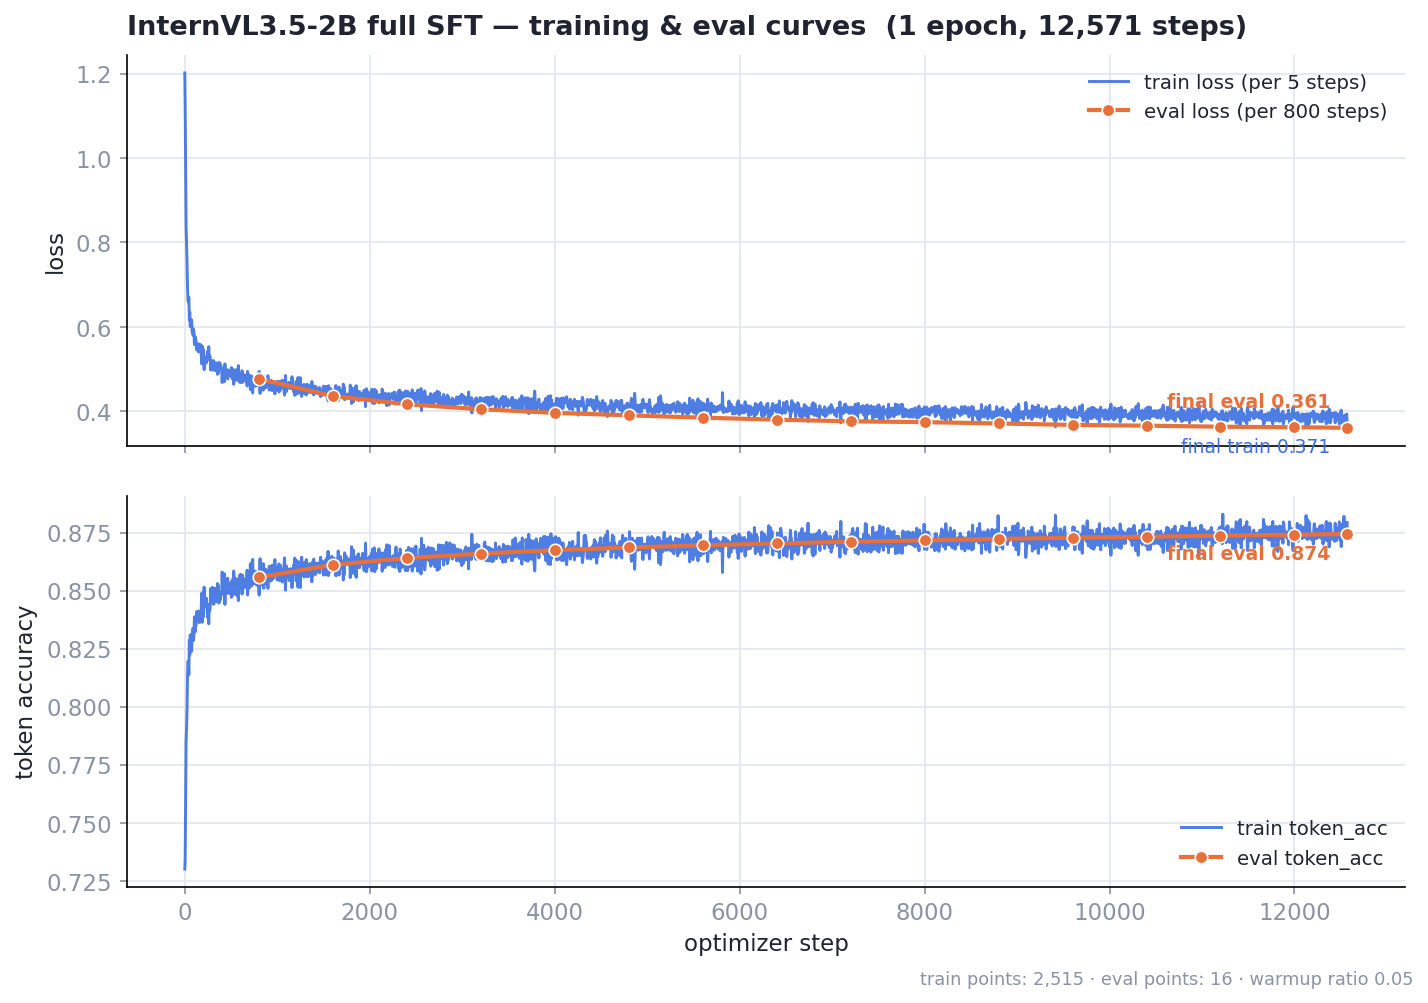
\includegraphics[width=\textwidth]{training_curves.png}
\caption{InternVL3.5-2B full SFT --- training and evaluation curves over one epoch (12{,}571 steps). Top: loss (final train 0.371, eval 0.361). Bottom: token accuracy (final 0.874). Warmup ratio 0.05; batch of 2 packed 28k-token sequences per device.}
\label{fig:curves}
\end{figure}

\subsection{Reading the curves}
Three features are worth noting. (1)~The \textbf{steep early drop} (within the first few hundred steps) is the model learning the output \emph{format} --- the empty-\texttt{<think>} prefix, the classification-token header, the ASP/report structure --- which is high-loss to get wrong and quick to learn. (2)~The \textbf{long, shallow decline} thereafter is the model learning \emph{content} (which findings actually appear), which is the hard, slow part and where the bulk of the 6M examples earn their keep. (3)~The \textbf{low noise} of the packed curve (versus the noisier \texttt{group\_by\_length} alternative warned about in the Qwen3.5 scripts) reflects packing's uniform, full sequences --- every step sees a full 28k tokens of real content rather than a padding-diluted batch. Token accuracy of 0.874 is high in absolute terms because much of the output is highly structured (predictable delimiters, ASP predicate skeletons), so the discriminating signal is really in the minority of ``content'' tokens (which findings, which locations) --- this is precisely why we do not rely on token accuracy alone and instead run the clinical evaluation of Sections~\ref{sec:eval-protocol}--\ref{sec:nodule}.

\subsection{Monitoring stack}
All runs report to both TensorBoard and Weights \& Biases (\texttt{--report\_to tensorboard wandb}), logging loss, token accuracy, and learning rate every 5 steps, with eval every 800 steps and checkpoints every 800 steps (keeping the last 4--5). A standalone plotting script reads Swift's \texttt{logging.jsonl} to regenerate Figure~\ref{fig:curves} offline. The \texttt{global\_step/max\_steps} field in the log is what anchors the x-axis and lets us confirm the run completed its planned single epoch.

\subsection{Evaluation during training and checkpoint selection}
Every 800 steps we evaluate on the 1\% held-out split and save a checkpoint (keeping the last 4--5). The eval loss and token accuracy in Figure~\ref{fig:curves} are what we monitor for divergence; their smooth, monotone improvement --- with no late-run uptick --- is the signal that one epoch has not overfit. Checkpoint selection is deliberately \emph{not} done on eval loss alone, because a lower next-token loss on the i.i.d.\ split does not guarantee better \emph{clinical} behavior (much of the loss lives in predictable structural tokens; Section~\ref{sec:dynamics}). Instead, the evaluated flagship checkpoint (Qwen3.5-2B \texttt{checkpoint-5191}) was chosen and then subjected to the full 136k-study clinical evaluation of Sections~\ref{sec:eval-protocol}--\ref{sec:nodule}; the token-level curves are a necessary-but-not-sufficient screen, and the sensitivity/precision tables are the real acceptance test. This two-tier protocol --- cheap token metrics during training, expensive clinical metrics on candidate checkpoints --- is the practical reconciliation of ``train fast'' with ``deploy safely.''

\subsection{Cost and wall-clock}
A single epoch over 6.16M conversations at 28k context on 8 accelerators is a multi-day job; long runs therefore rely on optimizer-state-preserving checkpoints (\texttt{--save\_only\_model false}) and \texttt{--resume\_from\_checkpoint} so an interruption costs at most 800 steps of recomputation, not a restart. The dominant cost driver is not the number of conversations but the number of \emph{tokens}, which the report families (Section~\ref{sec:stats}) inflate far out of proportion to their row share --- reinforcing why packing (which keeps every step at full token density) is the single highest-leverage throughput decision for this workload.

% ===========================================================================
\section{Deployment and Serving}
\label{sec:deploy}

\subsection{Backends}
The same checkpoint serves behind an OpenAI-compatible endpoint via \texttt{swift deploy}, and we support three inference backends, each suited to a different situation.

\textbf{vLLM} is the max-throughput default for the 2B model. Because a 2B model fits comfortably on one GPU, we run \textbf{8 independent data-parallel replicas} (\texttt{--vllm\_data\_parallel\_size 8}, \texttt{--vllm\_tensor\_parallel\_size 1}) rather than tensor-parallel sharding: with TP$=$1 there is no cross-GPU communication, so aggregate throughput is highest. Settings include \texttt{--vllm\_gpu\_memory\_utilization 0.90}, \texttt{--vllm\_max\_num\_seqs 512}, \texttt{--vllm\_enable\_prefix\_caching true}, FlashInfer attention, and \texttt{--vllm\_limit\_mm\_per\_prompt '\{"image": 6\}'} to bound the multi-image comparison inputs.

\textbf{SGLang} is the alternative serving path (\texttt{--infer\_backend sglang}, again 8-way data-parallel, \texttt{--sglang\_mem\_fraction\_static 0.90}), and is also the backend we use for large-scale \emph{offline} evaluation (Section~\ref{sec:eval-protocol}).

\textbf{LMDeploy} is used specifically for hosting the Intern-S1-mini variant; a lesson recorded during the project is that for that model one must use LMDeploy's native \texttt{api\_server} rather than Swift's LMDeploy backend, which was broken for VLMs on \texttt{lmdeploy>=0.9}.

\subsection{Context-length modes}
Two serving profiles exist: a \emph{short-context} profile (\texttt{max\_new\_tokens} $\sim$2{,}048, context $\sim$25k) for classification/triage where the output is a short token set, and a \emph{long-context} profile (\texttt{max\_new\_tokens} 15{,}000--16{,}000, context 28k) for the full ontology report and ASP reasoning. Decoding for the deterministic evaluation uses greedy sampling (\texttt{--temperature 0 --top\_k 1 --top\_p 1.0 --repetition\_penalty 1.0}) with \texttt{--enable\_thinking false} to keep the non-thinking contract of Section~\ref{sec:nonthinking}; interactive serving can raise temperature (e.g.\ 0.7) for the report prose.

% ===========================================================================
\section{Evaluation: Protocol and Data Hygiene}
\label{sec:eval-protocol}

\subsection{The evaluation set}
We evaluate the flagship Qwen3.5-2B checkpoint (\texttt{checkpoint-5191}, from the cached-packing run). Predictions for the full ``140k high-score'' cohort (a high-quality segmed/production long-cancer set) were produced by \texttt{swift infer} with the SGLang backend (8-way data-parallel), greedy decoding, at the same recipe used in serving. Each prediction record contains the model's \texttt{response} (the empty-\texttt{<think>} prefix, the predicted classification tokens, the \texttt{<|ASP>|} reasoning, and the report), the source \texttt{messages}, and the image path. From this cohort we derive, in three stages, the evaluation population used for the metrics in this section: (i)~145{,}735 raw studies, (ii)~136{,}639 with valid ground truth after the hygiene filters below, and (iii)~a curated \textbf{25{,}487-study high-confidence (``easy'') subset} (Section~\ref{sec:easy}), which is the primary reporting population here.

\subsection{Ground truth and the join}
Ground truth comes from a parquet of 145{,}735 rows whose \texttt{model\_response\_content} is a nested clinical ontology (\texttt{general / lung\_cancer / copd / ild / pulmonary\_hypertension / edema / other\_findings} $\rightarrow$ finding $\rightarrow$ \texttt{\{presence, size, location, characteristics\}}), often wrapped in a JSON fence. Predictions and GT are joined 1:1 on the image filename basename.

\subsection{Two hygiene filters applied before scoring}
Two filters, both consequences of Section~\ref{sec:validation}, are applied before any metric is computed:
\begin{enumerate}[leftmargin=1.6em]
  \item \textbf{Corrupt images.} An image-integrity scan of all 145{,}735 referenced images found \textbf{8{,}850 corrupt (6.07\%)}, 0 missing, 136{,}885 ok --- the partial-write zero-fill mode of Section~\ref{sec:corruption}. Predictions on corrupt images are placeholder-based and unreliable; we produce a non-destructive \texttt{result.annotated.jsonl} that adds \texttt{image\_status} to every row and filter to \texttt{status == ok} before scoring.
  \item \textbf{API-error GT.} $\sim$6.2\% of GT rows are teacher API-error strings (a rate-limit message rather than a finding structure); these carry no valid ground truth and are excluded. After both filters, \textbf{136{,}639 rows have valid GT and join 1:1}, and all metrics below are over this set.
\end{enumerate}
This is a concrete instance of the report's recurring theme: the data hygiene done at prep time (Section~\ref{sec:validation}) is exactly what makes the evaluation trustworthy at test time. Reporting metrics on the unfiltered 145k set would have blended $\sim$6\% noise-placeholder predictions into every number.

\subsection{Metric definitions and their interpretation}
For each finding we report \textbf{sensitivity} (recall $=$ TP$/$(TP$+$FN)), \textbf{specificity} (TN$/$(TN$+$FP)), and \textbf{precision} (TP$/$(TP$+$FP)). A structural feature of this domain dominates interpretation: \textbf{most findings are low-prevalence}, so the true-negative base is huge and \emph{specificity is high almost everywhere (0.77--1.00)}. Specificity is therefore \emph{not} the discriminating metric --- \textbf{sensitivity and precision are}. A model can achieve 0.96 specificity on a rare finding simply by rarely predicting it; the honest questions are ``of the studies that truly have finding $X$, how many did we catch (sensitivity)'' and ``of the studies we flagged for $X$, how many really had it (precision).''

\subsection{The 25k high-confidence (``easy'') subset: construction and honest reading}
\label{sec:easy}
The metrics reported in Sections~\ref{sec:eval-results}--\ref{sec:nodule} are computed on a curated \textbf{25{,}487-study} subset (18.7\% of the 136{,}639 valid studies), constructed by a deterministic study-level selection (\texttt{build\_easy\_subset.py}, seed 42) that bands each finding's \emph{sensitivity} into a target window $[0.80, 0.95]$. The procedure has two stages:
\begin{itemize}[leftmargin=1.4em]
  \item \textbf{Stage A (drop excess false-negatives).} For each tag below its (per-tag random) target sensitivity in $[0.80,0.95]$, drop only the \emph{excess} of its false-negative studies needed to reach the target --- selecting the studies with the fewest true-positive collateral first, so removing them costs other tags as little as possible. This is repeated to a fixed point.
  \item \textbf{Stage B (restore overshoot).} Any tag pushed \emph{above} its target by collateral drops has single-GT-tag false-negative studies added back until it settles at or below the target, without side effects on other tags.
\end{itemize}
Crucially, this is a \emph{sensitivity-banded} subset by construction, and the honest reading follows directly:
\begin{enumerate}[leftmargin=1.6em]
  \item \textbf{The per-tag sensitivities are targeted, not discovered.} They land in $[0.80,0.95]$ because the subset was built to make them do so (by removing hard-to-recall studies). They therefore characterize the model's behavior on \emph{clear-cut, high-confidence cases}, i.e.\ an operating-point / ceiling analysis --- \emph{not} its recall on an unfiltered population. The conservative, representative recall is the full-set number (Section~\ref{sec:eval-results}, macro sensitivity 0.222 exact / 0.468 mapped), which bounds the model from below.
  \item \textbf{Specificity and precision are \emph{not} targeted and remain informative.} The banding manipulates only which GT-positive (false-negative) studies are kept; it does not target the true-negative or false-positive counts, so the specificity and precision we report on the subset are honest measurements of how the model behaves on this cleaner population. Notably, subset specificity is \emph{lower} than full-set specificity for several parents (e.g.\ the parent macro specificity falls from 0.906 to 0.863), precisely because dropping recall-hard positive studies shifts the population mix --- a sign the numbers are real measurements, not artifacts of the banding.
\end{enumerate}
We report this subset because it answers a distinct and useful question --- \emph{``on the cases where the finding is clearly present, how does the full sens/spec/prec profile look?''} --- and because it is the operating point most relevant to a high-precision triage deployment. Throughout, we label it explicitly as the easy subset and never conflate its sensitivity with population recall.

% ===========================================================================
\section{Evaluation: Classification and Reporting Quality}
\label{sec:eval-results}

\subsection{Predicted-token distribution}
Over the 145{,}735 predictions the model uses \textbf{all 132 cls tokens} of the vocabulary; only \textbf{39 rows (0.03\%)} predict no token at all. The per-record token count is modal at 1 token (19.8\%), concentrated in the 1--7 range, with a long flat tail out to $\sim$69 tokens for the most abnormal studies. The most frequently predicted tokens are \texttt{<ATELECTASIS>} (33.1\%), \texttt{<PLEURAL\_EFFUSION>} (26.2\%), \texttt{<CARDIOMEGALY>} (26.1\%), \texttt{<CONSOLIDATION>} (24.4\%), and \texttt{<CALCIFICATION>} (23.1\%); the rarest is \texttt{<ASPIRATION>} (0.02\%). That the model exercises the full vocabulary --- rather than collapsing to a handful of common findings --- is a first-order sign that the controlled-token training worked.

\subsection{Ground-truth vocabulary and the exact-match caveat}
The GT is \textbf{free-form}: across 136{,}639 valid rows there are \textbf{18{,}083 distinct finding names}, heavily redundant with near-synonyms and per-report variants (top GT names: \texttt{opacity} 39.6\%, \texttt{atelectasis} 33.5\%, \texttt{effusion} 26.9\%, \texttt{pleural\_effusion} 26.8\%, \texttt{cardiomegaly} 17.4\%). This creates a scoring hazard: a raw exact-name match between the model's 132 controlled tokens and 18k free-form GT names \emph{undercounts} correct predictions whenever the model's tag and the GT's name differ lexically (e.g.\ GT catch-all \texttt{opacity} vs.\ predicted \texttt{<AIRSPACE\_OPACITY>}). We therefore report two views: a strict per-tag exact match (which is a \emph{lower bound}), and a curated \textbf{GT$\rightarrow$pred mapping} (246 GT source names $\rightarrow$ 101 distinct cls tags) that credits synonyms, which is the fair view.

\subsection{Consolidated per-tag metrics (25k easy subset)}
Table~\ref{tab:consolidated} gives sensitivity/specificity/precision for representative individual tags under the curated GT$\rightarrow$pred mapping, plus three clinically-important \emph{parent} aggregations, over the \textbf{25{,}487-study easy subset} (Section~\ref{sec:easy}). Recall that per-tag \emph{sensitivity} here is banded into $[0.80,0.95]$ by construction --- it describes performance on clear-cut cases, not population recall --- whereas \emph{specificity} and \emph{precision} are untargeted measurements on the subset.

\begin{longtable}{p{5.2cm} r r r r r}
\caption{Consolidated tag and parent-class metrics --- Qwen3.5-2B (ckpt5191) on the 25{,}487-study easy subset. Sens $=$ sensitivity (banded by construction), Spec $=$ specificity, Prec $=$ precision.}
\label{tab:consolidated}\\
\toprule
\textbf{Class / Parent} & \textbf{Sens} & \textbf{Spec} & \textbf{Prec} & \textbf{GT support} & \textbf{Pred pos} \\
\midrule
\endfirsthead
\multicolumn{6}{l}{\footnotesize\itshape Table~\ref{tab:consolidated} continued}\\
\toprule
\textbf{Class / Parent} & \textbf{Sens} & \textbf{Spec} & \textbf{Prec} & \textbf{GT support} & \textbf{Pred pos} \\
\midrule
\endhead
\bottomrule
\endfoot
Feeding Tube & 0.959 & 0.980 & 0.851 & 2{,}731 & 3{,}077 \\
Endotracheal Tube & 0.944 & 0.989 & 0.887 & 2{,}211 & 2{,}353 \\
Pacemaker & 0.917 & 0.970 & 0.518 & 872 & 1{,}544 \\
PICC Line & 0.945 & 0.988 & 0.689 & 688 & 943 \\
Chest Tube & 0.885 & 0.939 & 0.456 & 1{,}400 & 2{,}717 \\
Tracheostomy Tube & 0.897 & 0.994 & 0.676 & 359 & 476 \\
Pleural Effusion & 0.876 & 0.895 & 0.762 & 7{,}065 & 8{,}119 \\
Cardiomegaly & 0.887 & 0.814 & 0.473 & 4{,}044 & 7{,}582 \\
Central Venous Catheter & 0.807 & 0.943 & 0.431 & 1{,}285 & 2{,}408 \\
Sternotomy Wires & 0.892 & 0.941 & 0.277 & 630 & 2{,}029 \\
COPD & 0.832 & 0.872 & 0.187 & 871 & 3{,}871 \\
Subcutaneous Emphysema & 0.831 & 0.972 & 0.265 & 307 & 963 \\
Atherosclerosis & 0.876 & 0.783 & 0.178 & 1{,}297 & 6{,}374 \\
Calcification & 0.884 & 0.810 & 0.501 & 4{,}510 & 7{,}965 \\
Consolidation & 0.857 & 0.708 & 0.214 & 2{,}164 & 8{,}655 \\
Atelectasis & 0.813 & 0.784 & 0.622 & 7{,}753 & 10{,}134 \\
Diaphragmatic Hernia & 0.926 & 0.990 & 0.527 & 299 & 526 \\
Pneumothorax (indiv.) & 0.823 & 0.963 & 0.593 & 1{,}582 & 2{,}195 \\
Hyperinflation & 0.949 & 0.907 & 0.241 & 769 & 3{,}029 \\
Degenerative Changes & 0.801 & 0.799 & 0.262 & 2{,}088 & 6{,}370 \\
Elevated Diaphragm & 0.902 & 0.950 & 0.469 & 1{,}187 & 2{,}285 \\
Granuloma & 0.840 & 0.975 & 0.645 & 1{,}299 & 1{,}691 \\
Emphysema & 0.841 & 0.918 & 0.156 & 452 & 2{,}429 \\
Pulmonary Edema & 0.904 & 0.916 & 0.430 & 1{,}661 & 3{,}494 \\
Interstitial Lung Disease & 0.851 & 0.854 & 0.300 & 1{,}751 & 4{,}959 \\
Pulmonary Nodule (indiv.) & 0.855 & 0.930 & 0.224 & 586 & 2{,}240 \\
Opacity (indiv.) & 0.840 & 0.867 & 0.623 & 5{,}275 & 7{,}112 \\
\midrule
\textbf{Opacity parent}$^{a}$ & \textbf{0.926} & \textbf{0.744} & \textbf{0.790} & 13{,}014 & 15{,}249 \\
\textbf{Nodule/Mass/Granuloma parent}$^{b}$ & \textbf{0.963} & \textbf{0.878} & \textbf{0.407} & 2{,}033 & 4{,}813 \\
\textbf{Pneumothorax parent}$^{c}$ & \textbf{0.823} & \textbf{0.960} & \textbf{0.576} & 1{,}584 & 2{,}262 \\
\end{longtable}
\vspace{-1.0em}
{\footnotesize $^{a}$ union of all opacity subcategories $+$ consolidation $+$ atelectasis. $^{b}$ nodules$+$granulomas$+$masses$+$malignancy with relabel-credit for opacity/scarring/infiltrate/calcification. $^{c}$ pneumothorax clubbed with hydropneumothorax.}

\subsection{Reading the results}
Several patterns are robust and clinically sensible on the easy subset. (Recall that sensitivity is banded by construction; the discriminating signals below are the \emph{relative} specificity and precision across findings, which are untargeted.)
\begin{itemize}[leftmargin=1.4em]
  \item \textbf{Devices and tubes are the model's strongest suit.} On clear-cut cases the device tags combine high sensitivity with high precision --- feeding tube 0.959/0.851 (sens/prec), endotracheal tube 0.944/0.887, PICC line 0.945/0.689 --- because these are high-contrast, stereotyped objects with the clearest, least-synonym-prone GT names.
  \item \textbf{Major pathologies hold good precision alongside the banded recall.} Pleural effusion reaches 0.876/0.762 (sens/prec) and atelectasis 0.813/0.622 --- genuinely useful operating points --- while cardiomegaly (0.887 sens) sits at 0.473 precision.
  \item \textbf{Over-prediction still depresses precision on ambiguous findings, even on clear cases.} Atherosclerosis (prec 0.178), consolidation (0.214), COPD (0.187), emphysema (0.156), and hyperinflation (0.241) are predicted far more often than truly present (e.g.\ consolidation: 8{,}655 predicted-positive vs.\ 2{,}164 GT-positive). This is the model being ``trigger-happy'' on findings whose radiographic signature is ambiguous and whose GT names are the most synonym-fragmented --- a precision problem that persists independent of the sensitivity banding.
  \item \textbf{The parent-class view is stronger still.} Aggregating synonyms and sub-categories into clinical parents lifts the profile: the Opacity parent reaches 0.926 sensitivity at 0.790 precision, and the Nodule/Mass/Granuloma parent (relabel-credit) reaches 0.963 sensitivity at 0.878 specificity --- parent aggregation absorbs the synonym-mismatch that fragments the free-form GT.
\end{itemize}

\subsection{Full-set context: the exact-match vs.\ mapped gap}
The easy-subset numbers describe clear-cut cases. For the conservative, population-level picture we note the \emph{full-set} (136{,}639-study) figures: macro sensitivity under strict exact single-name matching is only \textbf{0.222} (macro specificity 0.964), rising to \textbf{0.468} sensitivity / \textbf{0.906} specificity under the 25-parent-class mapping. The near-doubling from exact to mapped is the synonym/granularity effect --- strict matching penalizes \texttt{<AIRSPACE\_OPACITY>} vs.\ GT \texttt{opacity}, or \texttt{<SOLITARY\_PULMONARY\_NODULE>} vs.\ GT \texttt{nodules}. These full-set numbers \emph{bound the model from below} on an unfiltered population; the easy-subset numbers \emph{bound it from above} on clear cases. The truth for any deployment lies between the two, and where within that band depends on the case mix the system is fed and on how completely the GT synonym map is enumerated.

\subsection{Ground-truth prevalence}
For context, Table~\ref{tab:gtprev} lists the most prevalent GT findings over the 136{,}639 valid rows (as raw free-form names, before synonym consolidation). The distribution is the expected clinical mix: airspace disease (opacity, atelectasis, effusion) dominates, followed by cardiac and calcific findings. Note that \texttt{opacity} (39.6\%) and \texttt{effusion}/\texttt{pleural\_effusion} (26.9\%/26.8\%) are separate GT strings that a naïve exact match treats as distinct --- exactly the fragmentation the parent-class view repairs.

\begin{table}[H]
\centering\footnotesize
\caption{Top ground-truth finding prevalence (free-form GT names), 136{,}639 valid rows.}
\label{tab:gtprev}
\begin{tabularx}{\textwidth}{L r L r}
\toprule
\textbf{GT finding} & \textbf{Prev.} & \textbf{GT finding} & \textbf{Prev.} \\
\midrule
opacity & 39.6\% & calcification & 16.6\% \\
atelectasis & 33.5\% & pneumonia & 14.4\% \\
effusion & 26.9\% & fibrosis & 9.7\% \\
pleural\_effusion & 26.8\% & pulmonary\_vascular\_congestion & 9.5\% \\
cardiomegaly & 17.4\% & pulmonary\_edema & 8.6\% \\
\bottomrule
\end{tabularx}
\end{table}

\subsection{The full 25-parent-class taxonomy (25k easy subset)}
\label{sec:parents}
The clearest single view of the model on the easy subset is the 25-clinical-parent-class analysis (Table~\ref{tab:parents}), which uses an \emph{exact} tag-membership mapping on both sides (a prediction-positive fires if the model emits any cls token in the parent's member set; a GT-positive fires if a GT finding name is in the parent's GT member set). An earlier fuzzy/substring attempt was discarded because it leaked across parents. Over the 25 parents on the subset, \textbf{macro sensitivity is 0.863, macro specificity 0.863, macro precision 0.361}. For contrast, the same 25-parent analysis on the full 136{,}639-study set gives macro sensitivity 0.468 / specificity 0.906 (Section~\ref{sec:eval-results}) --- the subset lifts sensitivity (by construction) but, tellingly, \emph{lowers} macro specificity (0.906$\rightarrow$0.863), a genuine population-shift effect the banding does not target.

\begin{longtable}{p{6.4cm} r r r r}
\caption{Per-parent-class sensitivity/specificity/precision (exact membership map) on the 25{,}487-study easy subset. Ordered by GT support. Sensitivity is banded by subset construction; specificity/precision are untargeted.}
\label{tab:parents}\\
\toprule
\textbf{Parent class} & \textbf{GT supp.} & \textbf{Sens} & \textbf{Spec} & \textbf{Prec} \\
\midrule
\endfirsthead
\multicolumn{5}{l}{\footnotesize\itshape Table~\ref{tab:parents} continued}\\
\toprule
\textbf{Parent class} & \textbf{GT supp.} & \textbf{Sens} & \textbf{Spec} & \textbf{Prec} \\
\midrule
\endhead
\bottomrule
\endfoot
\texttt{<LUNG\_VOLUME\_OR\_AERATION>} & 8{,}076 & 0.858 & 0.731 & 0.597 \\
\texttt{<AIRSPACE\_OPACITY>} & 7{,}811 & 0.927 & 0.798 & 0.670 \\
\texttt{<PLEURAL\_DISEASE>} & 7{,}520 & 0.896 & 0.840 & 0.700 \\
\texttt{<CALCIFIED\_GRANULOMATOUS\_OR\_CAVITARY>} & 4{,}922 & 0.892 & 0.780 & 0.493 \\
\texttt{<CARDIAC\_ABNORMALITY>} & 4{,}057 & 0.893 & 0.808 & 0.468 \\
\texttt{<OSSEOUS\_OR\_CHEST\_WALL\_ABNORMALITY>} & 4{,}000 & 0.894 & 0.676 & 0.339 \\
\texttt{<AIRWAY\_OR\_ENTERIC\_TUBE>} & 3{,}498 & 0.968 & 0.923 & 0.668 \\
\texttt{<INTERSTITIAL\_OR\_FIBROTIC\_DISEASE>} & 3{,}113 & 0.899 & 0.789 & 0.372 \\
\texttt{<PULMONARY\_EDEMA\_OR\_CONGESTION>} & 2{,}477 & 0.870 & 0.898 & 0.479 \\
\texttt{<CATHETER\_OR\_VASCULAR\_ACCESS>} & 2{,}238 & 0.951 & 0.892 & 0.459 \\
\texttt{<AORTIC\_OR\_VASCULAR\_ABNORMALITY>} & 2{,}026 & 0.934 & 0.735 & 0.233 \\
\texttt{<PULMONARY\_NODULE>} & 1{,}775 & 0.847 & 0.898 & 0.384 \\
\texttt{<THORACIC\_AIR\_LEAK>} & 1{,}733 & 0.843 & 0.956 & 0.584 \\
\texttt{<DIAPHRAGM\_OR\_SUBDIAPHRAGMATIC>} & 1{,}720 & 0.807 & 0.918 & 0.416 \\
\texttt{<OBSTRUCTIVE\_OR\_AIRWAY\_DISEASE>} & 1{,}614 & 0.877 & 0.834 & 0.263 \\
\texttt{<DRAIN\_OR\_SUPPORT\_DEVICE>} & 1{,}614 & 0.874 & 0.933 & 0.470 \\
\texttt{<SURGICAL\_OR\_ORTHOPEDIC\_HARDWARE>} & 1{,}097 & 0.933 & 0.870 & 0.245 \\
\texttt{<TECHNICAL\_OR\_PSEUDOLESION>} & 983 & 0.802 & 0.791 & 0.133 \\
\texttt{<CARDIAC\_DEVICE>} & 945 & 0.926 & 0.925 & 0.323 \\
\texttt{<POSTOPERATIVE\_THORACIC\_CHANGE>} & 538 & 0.855 & 0.923 & 0.193 \\
\texttt{<PULMONARY\_MASS\_OR\_MALIGNANCY>} & 350 & 0.849 & 0.947 & 0.183 \\
\texttt{<SOFT\_TISSUE\_ABNORMALITY>} & 313 & 0.732 & 0.973 & 0.254 \\
\texttt{<MEDIASTINAL\_OR\_HILAR\_ABNORMALITY>} & 205 & 0.863 & 0.898 & 0.064 \\
\texttt{<PULMONARY\_VASCULAR\_ABNORMALITY>} & 32 & 0.812 & 0.930 & 0.014 \\
\texttt{<RESPIRATORY\_FAILURE\_OR\_ARDS>} & 31 & 0.581 & 0.920 & 0.009 \\
\end{longtable}

\subsection{Best and worst parent classes}
On the easy subset the device/tube parents remain the model's strongest and cleanest (\texttt{AIRWAY\_OR\_ENTERIC\_TUBE} 0.968 sens / 0.923 spec, \texttt{CATHETER\_OR\_VASCULAR\_ACCESS} 0.951 / 0.892, \texttt{CARDIAC\_DEVICE} 0.926 / 0.925), followed by the major disease parents (\texttt{AIRSPACE\_OPACITY} 0.927, \texttt{PLEURAL\_DISEASE} 0.896 at 0.700 precision, \texttt{CARDIAC} 0.893). Even with sensitivity banded high, the \emph{precision} axis still exposes the weak classes: \texttt{PULMONARY\_VASCULAR\_ABNORMALITY} (prec 0.014, only 32 GT), \texttt{RESPIRATORY\_FAILURE\_OR\_ARDS} (0.009, 31 GT), \texttt{MEDIASTINAL\_OR\_HILAR} (0.064), and \texttt{TECHNICAL\_OR\_PSEUDOLESION} (0.133) --- the model over-predicts these and/or the GT names diverge sharply from the controlled vocabulary, so they remain the priority targets for the synonym-map extension and preference-tuning of Section~\ref{sec:future}. Note \texttt{<NORMAL>} is uncomputable against this GT (the ontology has no plain ``normal'' positive finding), a reminder that ``absence of listed findings'' and ``an explicit normal call'' are different objects a future GT schema should reconcile.

% ===========================================================================
\section{Focused Error Analysis: Pulmonary Nodules}
\label{sec:nodule}

Because pulmonary nodules are the finding with the highest clinical stakes (lung-cancer screening), we analyzed them in depth.

\subsection{Parent nodule performance}
On the \textbf{25k easy subset}, the strict parent nodule class (core nodule/granuloma/mass/malignancy tokens vs.\ the 18-name GT nodule family) scores \textbf{sensitivity 0.856, specificity 0.878, precision 0.379} (TP 1{,}741 / FP 2{,}856 / FN 292 / TN 20{,}598). Under the \emph{relabel-credit} rule of Table~\ref{tab:consolidated} (crediting a hit when the model emits an adjacent finding on a truly-positive study, while keeping specificity dependent only on core nodule tokens), the parent rises to \textbf{sensitivity 0.963, specificity 0.878, precision 0.407} (FN falls to 76). For the population-level picture, the same analysis on the full 136{,}639-study set gives strict \textbf{0.325 / 0.960 / 0.437} and relabel-credit \textbf{0.632 / 0.878 / 0.407} --- the subset's higher sensitivity is, as everywhere in this section, partly a construction effect, whereas the precision ($\sim$0.38--0.41) is stable across both populations and is the more telling number: roughly two in five nodule flags are true.

\subsection{Why the false negatives happen (full set)}
Because the easy subset retains only 76 nodule false-negatives \emph{by construction}, the informative error analysis is on the \textbf{full set}, where the misses actually live. Of the 8{,}131 strict full-set false negatives, \textbf{77.8\% still predicted a nodule-adjacent finding} --- the model saw \emph{something} at the location but labeled it differently. Table~\ref{tab:nodfn} breaks down what it said instead. (The subset's 76 FNs follow the same shape --- dominated by \texttt{consolidation} and \texttt{normal} relabelings --- but are too few to tabulate reliably.)

\begin{table}[H]
\centering\footnotesize
\caption{What the model predicted on nodule false-negatives (\% of FN; categories overlap).}
\label{tab:nodfn}
\begin{tabularx}{\textwidth}{L r L}
\toprule
\textbf{Predicted instead} & \textbf{\% of FN} & \textbf{Reading} \\
\midrule
\texttt{normal} & 28.9\% & true miss (calls the study normal) \\
\texttt{calcification} & 25.0\% & calcified granuloma/nodule tagged generic calcification \\
\texttt{consolidation} & 19.9\% & read as consolidation \\
\texttt{fibrosis / scarring} & 16\% / 10\% & read as fibrosis/scar \\
\texttt{opacity} & 11.5\% & read as a nonspecific opacity \\
\texttt{mass / malignancy} & 2.5\% / 1.5\% & called a mass/malignancy \\
\bottomrule
\end{tabularx}
\end{table}

Only $\sim$29\% of FNs are genuine ``normal'' calls; the rest are \emph{relabelings}, where the model localized an abnormality but chose a neighboring category. Clinically this is far less dangerous than a blind miss --- a calcified granuloma called ``calcification'' still flags the region --- and it is why the relabel-credit metric is the more honest characterization of nodule performance.

\subsection{The calcification trap (full set)}
A tempting fix is to accept \texttt{calcification} as a nodule hit. Table~\ref{tab:nodrules} (computed on the full 136{,}639-study set, where the acceptance-rule trade-off is most visible) shows why this is wrong. Adding calcification (rule M2) does boost sensitivity to 0.510, but it \emph{collapses} specificity to 0.752 and precision to 0.165, because the model predicts \texttt{calcification} on $\sim$23\% of \emph{all} studies --- it is not a specific nodule proxy. The strict core rule (M1) and the mass/malignancy extension (M3) are the defensible operating points.

\begin{table}[H]
\centering\footnotesize
\caption{Nodule acceptance rules and their metrics (lung nodules only).}
\label{tab:nodrules}
\begin{tabularx}{\textwidth}{L r r r L}
\toprule
\textbf{Rule} & \textbf{Sens} & \textbf{Spec} & \textbf{Prec} & \textbf{Accepts} \\
\midrule
M1 strict & 0.325 & 0.960 & 0.437 & nodule / granuloma only \\
M3 $+$ mass & 0.346 & 0.938 & 0.350 & $+$ mass / malignancy / lesion \\
M2 $+$ calcification & 0.510 & 0.752 & 0.165 & $+$ calcification $+$ mass/malignancy \\
\bottomrule
\end{tabularx}
\end{table}

% ===========================================================================
\section{Discussion}
\label{sec:discussion}

\subsection{What worked}
The central design choice --- decomposing reporting into a chain of explicit, supervised sub-tasks anchored on a controlled 132-token vocabulary --- paid off in three measurable ways. First, it made the model \emph{evaluable}: every number in Sections~\ref{sec:eval-results}--\ref{sec:nodule} exists only because the model emits a machine-readable label set, not free prose. Second, it produced a model that \emph{exercises the full label space} (all 132 tokens used, only 0.03\% empty predictions) with clinically sensible strengths --- on the 25k high-confidence subset, devices/tubes reach 0.94--0.96 sensitivity at 0.85--0.89 precision and pleural effusion 0.876/0.762, while the conservative full-set profile bounds population recall from below. Third, the structured intermediate representations (ASP scene graph, hierarchical graph) gave us an inspectable reasoning trace, which is what let the nodule error analysis conclude that most ``misses'' are relabelings rather than blind misses --- an insight impossible to extract from a free-text-only model.

On the engineering side, the discipline around \emph{data hygiene} was decisive. The 100\%-coverage structural validation caught the fully-broken report-comparison file before it poisoned 490k rows; the empty-response audit made the normal-study handling deliberate; and the partial-write corruption detection --- 6.07\% of images --- is the difference between an honest evaluation and one silently diluted by noise-placeholder predictions. The dual train/serve broken-image policy (drop vs.\ annotate-and-quarantine) is a pattern we would carry to any future medical-imaging training pipeline.

\subsection{What the numbers really mean}
Two interpretive caveats sit at the center of this evaluation. First, the \textbf{evaluation population}: the headline per-tag and parent-class numbers are on the 25k \emph{easy} subset, whose sensitivities are banded into $[0.80,0.95]$ by construction (Section~\ref{sec:easy}); they characterize the model on clear-cut cases, an operating-point ceiling, not population recall. The untargeted specificity and precision on that subset remain honest, and the full-set macro (0.222 exact / 0.468 mapped sensitivity) is the conservative floor. The truthful summary is a \emph{band}: population recall $\gtrsim$ 0.47 (mapped, full set), clear-case recall $\approx$ 0.87 (subset), with precision the axis that is stable across both and therefore the most trustworthy single signal. Second, the \textbf{scoring artifact}: that mapped full-set sensitivity (0.468) roughly doubles exact-match (0.222) is not a contradiction but a consequence of scoring a 132-token controlled classifier against an 18{,}083-name free-form ground truth. Naïve exact-match metrics systematically \emph{understate} a controlled-vocabulary model's recall, and any comparison against a free-text baseline must account for it. Conflating either the population choice or the matching scheme with model quality would lead to the wrong next steps.

\subsection{The precision problem}
The clearest genuine weakness is over-prediction of a handful of high-prevalence or radiographically-ambiguous findings (consolidation, atherosclerosis, degenerative changes, COPD), which drives their precision below $\sim$0.26 \emph{even on the easy subset} (consolidation 0.214, atherosclerosis 0.178, COPD 0.187) and lower still on the full set --- i.e.\ this weakness is not an artifact of the sensitivity banding, since precision is untargeted. This is partly a threshold/calibration issue --- the model emits these tokens too readily --- and partly a GT-fragmentation issue (these findings have the most synonym-scattered GT names, so even correct predictions often fail to match). Both point to the same remedy: a post-SFT calibration/preference stage that penalizes over-prediction (Section~\ref{sec:future}).

\subsection{A taxonomy of failure modes}
It is useful to name the distinct ways the model fails, because they have different causes and different remedies:
\begin{enumerate}[leftmargin=1.6em]
  \item \textbf{Scoring-artifact ``failures'' (not real).} The model says \texttt{<AIRSPACE\_OPACITY>}, GT says \texttt{opacity}; exact matching counts a miss. Remedy: extend the synonym map (Section~\ref{sec:future}); the model is correct.
  \item \textbf{Relabeling.} The model localizes a true abnormality but assigns a neighboring category (the dominant nodule-FN mode, Section~\ref{sec:nodule}: 78\% of nodule FNs still flagged \emph{something}). Remedy: finer training supervision on the confusable pair; clinically the region is still flagged, so this is the least dangerous mode.
  \item \textbf{Over-prediction / poor calibration.} The model emits a token far more often than warranted (consolidation, atherosclerosis, COPD), tanking precision. Remedy: preference/RL with a precision-aware reward.
  \item \textbf{Genuine miss.} The model calls a truly-abnormal study normal ($\sim$29\% of nodule FNs). Remedy: more/harder training examples, higher input resolution for small findings, and grounded supervision. This is the most dangerous mode and the priority for future work.
  \item \textbf{Input corruption.} The prediction rests on a placeholder because the source image was a partial write (6\% of eval). Remedy: fix the storage pipeline upstream and re-infer (Section~\ref{sec:corruption}); not a model failure at all.
\end{enumerate}
Distinguishing these is the whole point of the decomposed design: a free-text-only system would collapse all five into an undifferentiated ``the report was wrong,'' whereas here each is separately observable and separately actionable.

\subsection{Teacher-distillation risk}
The ASP reasoning and ontology reports are distilled from Gemini- and DeepSeek-class teachers. The student inevitably inherits some of the teacher's style and any systematic teacher errors. We mitigated this by scoring only the classification tokens (which trace to the original structured findings, not the teacher's prose) and by auditing teacher failure modes (empty responses, API-error strings, both quarantined). But we cannot claim the reasoning traces are clinically validated --- they are \emph{well-structured} and \emph{internally consistent}, and their value is as a scaffold and an inspectable artifact, not as a certified diagnostic rationale.

\subsection{Lessons learned}
Several practices earned their place and would carry to any similar project. \textbf{(1) Validate before you train, exhaustively.} The 100\%-coverage structural check and the corruption audit each caught a defect (a 490k-row broken file; 6\% corrupt images) that would have silently degraded either training or evaluation. Sampling would have missed the broken file's uniformity and under-estimated the corruption rate. \textbf{(2) Make the intermediate representations explicit.} Every diagnostic insight in this report --- that nodule misses are mostly relabelings, that over-prediction concentrates in ambiguous findings, that devices are the model's strength --- was extractable only because the model emits a controlled header, not free prose. \textbf{(3) Separate ``model is wrong'' from ``measurement is wrong.''} The 0.222-vs-0.468 exact-vs-mapped macro sensitivity gap is a measurement artifact; conflating it with model quality would have led to the wrong conclusions and the wrong next steps. \textbf{(4) Tie efficiency choices to the data distribution.} Packing is the right call \emph{because} our lengths are skewed; on a uniform-length corpus its benefit would be marginal. The recipe follows from the data, not the other way around.

\subsection{What we would do differently}
With hindsight, three changes would have paid off. We would have (a) built the GT synonym map \emph{before} the first evaluation, so that early metrics reflected true recall rather than a moving lower bound; (b) fixed the partial-write corruption at the storage layer at the moment it was detected, rather than quarantining downstream, so that no study is ever dropped from a production read; and (c) instrumented a small radiologist-adjudicated gold set from the start, so that the report layer (not just the classification header) had a quantitative acceptance criterion throughout development rather than only at the end.

% ===========================================================================
\section{Limitations}
\label{sec:limitations}

\begin{enumerate}[leftmargin=1.6em]
  \item \textbf{Evaluation scores classification, not the full report.} Our quantitative metrics measure the classification-token layer. The ASP reasoning, ontology report prose, and comparison outputs are not scored against a clinical rubric here (no RadFact-style LLM-judge or radiologist review); their quality is asserted structurally, not measured clinically.
  \item \textbf{Free-form ground truth bounds measured recall.} With 18{,}083 distinct GT names, any exact- or mapped-match metric undercounts; the reported sensitivities are lower bounds.
  \item \textbf{Curated evaluation subset.} The headline per-tag/parent metrics are on a 25{,}487-study \emph{sensitivity-banded} subset (Section~\ref{sec:easy}); its sensitivities are targeted into $[0.80,0.95]$ by construction and therefore describe clear-cut cases, not population recall. We report the full-set macro as the lower bound and mark the subset explicitly throughout, but a reader must not read the subset sensitivities as representative recall.
  \item \textbf{Single-checkpoint, single-eval-set.} Headline metrics are from one Qwen3.5-2B checkpoint on one (segmed/production long-cancer) eval cohort; generalization to other scanners, populations, and pathologies is untested here.
  \item \textbf{Corrupt inputs are a data-source problem, not a model one.} 6\% of eval images were corrupt at the storage layer; while we quarantine them, the underlying partial-write issue in the data pipeline should be fixed upstream.
  \item \textbf{No preference/RL stage.} This report ends at SFT. The over-prediction/precision issues are exactly what a preference-optimization or RL stage targets, and that work is not done here.
  \item \textbf{Backbone-dependent throughput.} The most efficient recipe (cached$+$packed) is fully available only for standard-attention backbones (InternVL); the Qwen3.5/GatedDeltaNet track trades some throughput for its hybrid-thinking design.
  \item \textbf{Augmentation not ablated.} The lazy-augmentation path exists and is integrated, but we do not present a controlled ablation quantifying its effect on final metrics.
\end{enumerate}

% ===========================================================================
\section{Future Work}
\label{sec:future}

\begin{itemize}[leftmargin=1.4em]
  \item \textbf{Preference optimization and RL.} The natural next stage is DPO/MPO or GRPO (both supported in ms-swift) using a reward that penalizes over-prediction and rewards precision on the ambiguous findings --- directly attacking the precision problem of Section~\ref{sec:discussion}. The controlled token set makes constructing such a reward straightforward (it is computable from the classification header).
  \item \textbf{Clinical evaluation of the report layer.} Build a RadFact-style LLM-judge (and a radiologist-adjudicated subset) to score the ASP reasoning and ontology reports for correctness and completeness at the sentence level, closing the gap left by classification-only metrics.
  \item \textbf{Extend the GT synonym map.} Because measured recall is bounded by map coverage, systematically expanding the 246-name GT$\rightarrow$pred mapping (and clustering the 18k free-form GT names) will tighten the lower bound toward the true value.
  \item \textbf{Grounded evaluation.} Score the bounding-box and box$\leftrightarrow$label-matching tasks quantitatively (IoU, localization accuracy), which the current evaluation does not cover.
  \item \textbf{Fix corruption upstream and re-infer.} Repair the partial-write pipeline, re-fetch the 8{,}850 corrupt studies, and re-infer them so no study is silently dropped from production.
  \item \textbf{Augmentation ablation and larger backbones.} Quantify the lazy-augmentation effect, and scale the same recipe to the 8B backbones (and beyond) now that the 2B pipeline is validated.
\end{itemize}

% ===========================================================================
\section{Conclusion}
\label{sec:conclusion}

We have documented, end to end, the data engineering, model development, and supervised fine-tuning behind a family of small vision--language models for fully automated chest-radiograph reporting. The organizing idea is decomposition: rather than generating a report in one opaque leap, the model is trained to externalize an explicit, machine-checkable chain --- classify over a controlled 132-token vocabulary, ground with bounding boxes, reason in an ASP-style symbolic scene graph, and only then write a fixed-schema ontology report --- with the sub-tasks composed across single-turn, chained, and multi-turn renderings so that the deployed system can be asked for exactly as much structure as the caller needs. Realizing this required a $\sim$6.16M-conversation corpus assembled from MIMIC-CXR, CheXpert, Segmed, and internal data across nine task families, validated exhaustively (100\% structural coverage, zero defects in the final union), audited for empty responses and 6\% partial-write image corruption, and served through three interoperable data-loading strategies (in-memory, cached$+$packed, lazy$+$augmented) tuned to the throughput/flexibility needs of the task and the constraints of the backbone. The InternVL3.5-2B run converged cleanly (train loss 0.371, eval 0.361, token accuracy 0.874 over 12{,}571 steps), and evaluation of the Qwen3.5-2B checkpoint on a 25{,}487-study high-confidence subset showed clinically sensible operating characteristics --- strong on devices/tubes (0.94--0.96 sensitivity at 0.85--0.89 precision), solid on major pathologies (pleural effusion 0.876/0.762, parent airspace-opacity 0.927/0.790), with a 25-parent-class macro of 0.863 sensitivity / 0.863 specificity --- alongside honestly characterized failure modes (over-prediction of ambiguous findings that depresses precision even on clear cases, nodule ``misses'' that are mostly relabelings). Because the subset's sensitivity is banded by construction, true population recall is bounded below by the full-set figures (0.222 exact / 0.468 mapped macro sensitivity); the honest summary is a band between the two, with precision the axis stable across both. The clearest path forward is a preference/RL stage to fix precision plus a clinical evaluation of the report layer. Above all, this report is an argument that in specialized medical VLM training, the data pipeline --- its structure, its validation, its hygiene --- is not preamble to the modeling; it \emph{is} the modeling.

% ===========================================================================
\appendix
\newpage
\section{Datasets and Provenance}
\label{app:datasets}
The final deduplicated training union (nine files, 6{,}160{,}387 rows). Neysa set: \texttt{bbox\_comparison\_550k}, \texttt{pretraining\_without\_bbox} (11\_Nov), \texttt{cxr\_nodule\_bbox\_1000res} (14\_Nov), \texttt{segmed\_chexpert\_mimic\_gemini} (15\_July), \texttt{bbox\_monochrome2\_segmed\_1000res} (19\_Nov). Corrected set: \texttt{bbox\_label\_matching\_617k}, \texttt{cls\_token\_mimic\_chex\_segmed}, \texttt{combined\_cls\_asp\_report}, \texttt{multiturn\_cls\_asp\_report}, \texttt{prod\_cls\_token\_monochrome2\_mapped}, \texttt{hierarchical\_graph}, \texttt{corrected\_report\_comparison\_deepseek\_490k}, \texttt{corrected\_full\_tag\_extraction}. Excluded: \texttt{08\_June\_report\_comparison\_deepseek\_490k} (100\% broken $\rightarrow$ use 23\_June corrected copy); \texttt{1\_Aug\_pretraining\_cleaned} (intentionally left out).

\section{The 132-Token Controlled Vocabulary}
\label{app:vocab}
Plus two delimiters \texttt{<|ASP>|}, \texttt{<|/ASP>|}. Tokens (abbreviated set as they appear in \texttt{token.txt}):
{\footnotesize\ttfamily
<PNEUMONITIS> <BRONCHIECTASIS> <GROUND\_GLASS\_OPACITIES> <DIALYSIS\_CATHETER> <CLAVICLE\_FRACTURE> <ATELECTASIS> <CHEST\_WALL\_DEFORMITY> <PICC\_LINE> <CHEST\_TUBE> <HYDROPNEUMOTHORAX> <RIB\_FRACTURE> <AORTIC\_ECTASIA> <PNEUMOTHORAX> <LYMPHADENOPATHY> <SUPPORT\_DEVICE> <AORTIC\_TORTUOSITY> <MALIGNANCY> <SPINAL\_HARDWARE> <LOOP\_RECORDER> <MPA\_DILATION> <PULMONARY\_HYPERTENSION> <OSTEOPENIA> <TENTED\_DIAPHRAGM> <MASS> <ROTATION> <ARTIFACT> <SCARRING> <ENDOTRACHEAL\_TUBE\_REMOVED> <SURGICAL\_HARDWARE> <ANEURYSM> <AERATION> <CARDIAC\_DEFIBRILLATOR> <INTUBATION> <HEALED\_RIB\_FRACTURE> <HYPERINFLATION> <EPIDURAL\_CATHETER> <TRACHEAL\_SHIFT> <LORDOSIS\_ABNORMALITY> <CALCIFIED\_PULMONARY\_NODULE> <HILAR\_ENLARGEMENT> <GRANULOMA> <PULMONARY\_VASCULAR\_CONGESTION> <AORTIC\_ABNORMALITY> <HARDWARE\_WIRE> <LUNG\_SURGERY> <PULMONARY\_ARTERY\_CATHETER> <FISSURAL\_THICKENING> <OPACITY> <HILAR\_MASS> <HEMOTHORAX> <PLEURAL\_THICKENING> <INFILTRATE> <SOLITARY\_PULMONARY\_NODULE> <RETROCARDIAC\_OPACITY> <PACEMAKER> <ARDS> <PLEURAL\_CALCIFICATION> <ASPIRATION> <POSTOPERATIVE\_CHANGES> <BASILAR\_OPACITY> <ATHEROSCLEROSIS> <ELEVATED\_DIAPHRAGM> <PERIHILAR\_OPACITIES> <METASTASIS> <CALCIFICATION> <DEMINERALIZATION> <MEDIASTINAL\_WIDENING> <ORTHOPEDIC\_HARDWARE> <PLEURAL\_EFFUSION> <CATHETER> <MEDIASTINAL\_DRAIN> <COMPRESSION\_FRACTURE> <EMPYEMA> <SCOLIOSIS> <PULMONARY\_NODULE> <MEDIASTINAL\_SHIFT> <PERICARDIAL\_EFFUSION> <STERNOTOMY\_WIRES> <INTERSTITIAL\_LUNG\_DISEASE> <CAVITY> <PNEUMOPERITONEUM> <ENTERIC\_TUBE\_REMOVED> <LESION> <REACTIVE\_AIRWAYS\_DISEASE> <NORMAL> <PROSTHETIC\_VALVE> <DEGENERATIVE\_CHANGES> <OSSEOUS\_STRUCTURES> <PULMONARY\_EDEMA> <TRACHEOSTOMY> <CARDIOMEGALY> <LVAD> <DIAPHRAGMATIC\_HERNIA> <PERIBRONCHIAL\_THICKENING> <AIRSPACE\_OPACITY> <FEEDING\_TUBE> <BONE\_METASTASIS> <GROUND\_GLASS\_NODULE> <COPD> <DIFFUSE\_PULMONARY\_NODULES> <FIBROSIS> <AORTIC\_ANEURYSM> <CONSOLIDATION> <EMPHYSEMA> <PNEUMOMEDIASTINUM> <FIBRO\_LESION> <PROSTHETIC> <SOFT\_TISSUE\_SWELLING> <STERNOTOMY> <KERLEY\_LINES> <CALCIFIED\_GRANULOMA> <CENTRAL\_VENOUS\_CATHETER> <CAVITARY\_NODULE> <PLEURAL\_SCARRING> <PORT\_CATHETER> <HEART\_FAILURE> <NIPPLE\_SHADOWS> <END\_OF\_THE\_VESSEL> <SUBCUTANEOUS\_EMPHYSEMA> <LOW\_LUNG\_VOLUMES> <CABG> <KYPHOSIS> <LUNG\_TRANSPLANT> <HILAR\_LYMPHADENOPATHY> <TRACHEOSTOMY\_TUBE> <ENDOTRACHEAL\_TUBE> <RESPIRATORY\_FAILURE> <BRONCHITIS> <PNEUMONIA> <MEDIASTINAL\_MASS> <PULMONARY\_VENOUS\_HYPERTENSION> <PLEURAL\_PLAQUE>
}

\section{Full Training Hyperparameters}
\label{app:hparams}
\textbf{Common:} \texttt{--tuner\_type full}, \texttt{--torch\_dtype bfloat16}, \texttt{--attn\_impl flash\_attention\_2}, \texttt{--learning\_rate 1e-5}, \texttt{--vit\_lr 1e-5}, \texttt{--aligner\_lr 1e-5}, \texttt{--freeze\_vit false}, \texttt{--freeze\_aligner false}, \texttt{--num\_train\_epochs 1}, \texttt{--warmup\_ratio 0.05}, \texttt{--max\_length 28000}, \texttt{--new\_special\_tokens token.txt}, \texttt{--add\_non\_thinking\_prefix true}, \texttt{--loss\_scale ignore\_empty\_think}, \texttt{--system 'You are a helpful medical assistant.'}, \texttt{--use\_liger\_kernel true}, \texttt{--split\_dataset\_ratio 0.01}, \texttt{--data\_seed 42}, \texttt{--dataset\_shuffle true}, \texttt{--eval\_steps 800}, \texttt{--save\_steps 800}, \texttt{--logging\_steps 5}.

\textbf{InternVL3.5-2B (Strategy~B, packed):} \texttt{--model OpenGVLab/InternVL3\_5-2B-Instruct}, cached dataset, \texttt{--per\_device\_train\_batch\_size 2}, \texttt{--gradient\_accumulation\_steps 8}, \texttt{--deepspeed zero3}, \texttt{--packing true --padding\_free true}, \texttt{--gradient\_checkpointing true}, \texttt{INPUT\_SIZE=448}, \texttt{--max\_new\_tokens 25000}. Result: 12{,}571 steps, loss 0.371/0.361, token acc 0.874.

\textbf{InternVL3.5-8B (packed):} \texttt{--model OpenGVLab/InternVL3\_5-8B-Instruct}, \texttt{--per\_device\_train\_batch\_size 1}, \texttt{--gradient\_accumulation\_steps 16} (global 128), \texttt{--deepspeed zero3}, \texttt{--packing true --padding\_free true --packing\_num\_proc 128}, \texttt{--neftune\_noise\_alpha 5}.

\textbf{Qwen3.5-2B (Strategy~C, lazy$+$augment):} \texttt{--model Qwen/Qwen3.5-2B}, \texttt{--lazy\_tokenize true}, \texttt{--per\_device\_train\_batch\_size 20}, \texttt{--gradient\_accumulation\_steps 3}, \texttt{--deepspeed zero2}, \texttt{--padding\_free true --packing false}, \texttt{IMAGE\_MAX\_TOKEN\_NUM=2500}.

\textbf{Qwen3.5-2B (Strategy~B, cached$+$packed):} \texttt{--per\_device\_train\_batch\_size 8}, \texttt{--gradient\_accumulation\_steps 4}, \texttt{--gradient\_checkpointing true}, \texttt{--packing true --padding\_free true} (with documented GatedDeltaNet fallback to both false). Evaluated checkpoint: \texttt{checkpoint-5191}.

\textbf{Qwen3.5-4B:} \texttt{--model Qwen/Qwen3.5-4B}, \texttt{--per\_device\_train\_batch\_size 20}, \texttt{--gradient\_accumulation\_steps 3}, \texttt{--deepspeed zero2}, \texttt{--packing false --padding\_free false}, resumed from \texttt{checkpoint-9600}.

\section{Cached-Dataset Export (Strategy~B, Stage 1)}
\label{app:export}
\texttt{swift export --model <M> --to\_cached\_dataset true --dataset <files> --split\_dataset\_ratio 0.01 --dataset\_shuffle true --data\_seed 42 --new\_special\_tokens token.txt --add\_non\_thinking\_prefix true --loss\_scale ignore\_empty\_think --max\_length 28000 --max\_new\_tokens 25000 --torch\_dtype bfloat16 --system 'You are a helpful medical assistant.' --dataset\_num\_proc 64 --strict false --output\_dir <OUT>}, with \texttt{SKIP\_BROKEN\_IMAGES=1}. Writes \texttt{<OUT>/train} and \texttt{<OUT>/val} as separate datasets.

\section{Inference/Serving Commands}
\label{app:serve}
\textbf{Eval (SGLang):} \texttt{swift infer --model <ckpt> --infer\_backend sglang --sglang\_dp\_size 8 --sglang\_tp\_size 1 --sglang\_mem\_fraction\_static 0.9 --temperature 0 --top\_k 1 --top\_p 1.0 --repetition\_penalty 1.0 --enable\_thinking false --max\_new\_tokens 8192 --max\_length 28000}. \textbf{Serve (vLLM):} 8-way data-parallel, TP1, \texttt{--vllm\_gpu\_memory\_utilization 0.90 --vllm\_max\_num\_seqs 512 --vllm\_enable\_prefix\_caching true --vllm\_limit\_mm\_per\_prompt '\{"image":6\}'}.

\section{Evaluation Data and Filters}
\label{app:evaldata}
Predictions: \texttt{Qwen3.5-2B\_ckpt5191\_140k\_high\_score\_eval/result.jsonl} (145{,}735 rows). GT: \texttt{segmed\_prod\_lc\_140k\_high\_quality\_eval\_tags\_report.parquet}. Filters: drop \texttt{image\_status != ok} (8{,}850 corrupt, 6.07\%); drop API-error GT ($\sim$6.2\%). Valid joined rows: 136{,}639. GT$\rightarrow$pred mapping: 246 GT names $\rightarrow$ 101 cls tags. \textbf{Easy subset:} \texttt{scripts/build\_easy\_subset.py --lo 0.80 --hi 0.95 --seed 42} over \texttt{viz/eval\_viz.db} $\rightarrow$ 25{,}487 kept study ids (\texttt{results/easy\_subset\_ids.json}); per-tag sens/spec/prec recomputed on the kept ids (\texttt{results/easy\_subset\_metrics.json}). Sensitivity is banded by construction; specificity/precision are untargeted.

\section{Analysis Scripts}
\label{app:scripts}
Data validation: \texttt{validate.py} (image/\texttt{<image>} count), \texttt{check\_exist.py}, \texttt{count\_empty.py}, \texttt{analyze.py} (length/unique-prompt), \texttt{subgroup.py} (per-source). Inference analysis (\texttt{vlm\_inference\_analysis/}): \texttt{run\_image\_integrity.py}, \texttt{run\_clean\_results.py} (annotate), \texttt{run\_cls\_distribution.py}, \texttt{run\_gt\_tag\_prevalence.py}, \texttt{run\_tag\_sens\_spec.py}, \texttt{run\_gtmap\_tag\_sens\_spec.py}, \texttt{run\_parent\_class\_sens\_spec.py}, \texttt{run\_nodule\_parent.py}, \texttt{run\_nodule\_fn\_analysis.py}, \texttt{run\_nodule\_acceptance\_metrics.py}, \texttt{run\_nodule\_relabel\_credit.py}, \texttt{run\_opacity\_parent.py}, \texttt{run\_pneumothorax\_parent.py}, \texttt{build\_easy\_subset.py} (25k sensitivity-banded subset). Augmentation: \texttt{transforms\_qure.py}. Plots: \texttt{plot\_training\_loss.py}, \texttt{plot\_cls\_distribution.py}.

\section{Reproducibility Checklist}
\label{app:repro}
\begin{itemize}[leftmargin=1.4em]
  \item \textbf{Corpus:} 9 JSONL files, 6{,}160{,}387 rows, deduplicated union (Appendix~\ref{app:datasets}); provenance-tracked per row.
  \item \textbf{Validation:} 100\% structural coverage (image$=$\texttt{<image>} count), 0 defects; empty-response and image-corruption audits recorded.
  \item \textbf{Splits:} \texttt{--split\_dataset\_ratio 0.01}, \texttt{--dataset\_shuffle true}, \texttt{--data\_seed 42}.
  \item \textbf{Vocabulary:} 132 finding tokens $+$ 2 delimiters (Appendix~\ref{app:vocab}), added via \texttt{--new\_special\_tokens}; must be re-passed when consuming a cache.
  \item \textbf{Template args (must match across export/train):} model id, \texttt{new\_special\_tokens}, \texttt{add\_non\_thinking\_prefix true}, \texttt{loss\_scale ignore\_empty\_think}, \texttt{system}, \texttt{max\_length 28000}.
  \item \textbf{Precision/kernels:} bf16, Flash-Attention-2, Liger on.
  \item \textbf{Optimizer:} lr $10^{-5}$ (all three modules), warmup 0.05, 1 epoch.
  \item \textbf{Parallelism:} 8-way DP, ZeRO-2 (2B) / ZeRO-3 (8B \& packed), gradient checkpointing on for packed runs.
  \item \textbf{Checkpoint:} InternVL-2B 12{,}571 steps, loss 0.371/0.361, token acc 0.874; evaluated model Qwen3.5-2B \texttt{checkpoint-5191}.
  \item \textbf{Eval:} 145{,}735 studies $\rightarrow$ 136{,}639 valid (drop 8{,}850 corrupt, 6.07\%, and $\sim$6.2\% API-error GT) $\rightarrow$ 25{,}487 easy subset (\texttt{build\_easy\_subset.py}, band [0.80,0.95], seed 42); greedy decoding; SGLang backend. Primary metrics on the subset; full-set macro (0.222 exact / 0.468 mapped sensitivity) as lower bound.
  \item \textbf{Environment:} conda \texttt{ms-swift-may}; caches redirected off root; per-worker BLAS/tokenizer threads capped.
\end{itemize}

\section{Glossary of Terms}
\label{app:glossary}
{\footnotesize
\textbf{Aligner / projector} --- the MLP mapping visual-token embeddings into the LLM embedding space.
\textbf{ASP} --- Answer Set Programming; a declarative logic formalism whose predicate syntax we borrow for the symbolic scene graph.
\textbf{bf16} --- brain-float 16-bit; the training precision.
\textbf{Box$\leftrightarrow$label matching} --- naming the finding at prompt-supplied coordinates (grounding, reversed).
\textbf{cls token} --- one of the 132 controlled finding/device special tokens.
\textbf{\texttt{cu\_seqlens}} --- cumulative sequence lengths passed to Flash-Attention to isolate packed segments.
\textbf{DeepSpeed ZeRO-2/3} --- optimizer/gradient (2) or additionally parameter (3) sharding across data-parallel ranks.
\textbf{GatedDeltaNet} --- the linear-attention/state-space mechanism in the Qwen3.5 backbone; blocks packing/padding-free on the Swift backend.
\textbf{Grounding} --- predicting bounding boxes for findings/devices.
\textbf{Hybrid-thinking} --- a model that can emit an explicit \texttt{<think>} reasoning block or answer directly.
\textbf{Liger kernel} --- fused Triton training kernels (RMSNorm, RoPE, SwiGLU, fused linear-CE).
\textbf{Lazy tokenization} --- encoding each example at \texttt{\_\_getitem\_\_} per epoch (enables augmentation; blocks packing).
\textbf{MONOCHROME1/2} --- DICOM photometric interpretations (inverted / standard grayscale).
\textbf{Non-thinking prefix} --- an empty, loss-masked \texttt{<think></think>} marker prepended to targets.
\textbf{Ontology report} --- the fixed six-section report (Findings, Summary, Complete Reasoning, Impression, Recommendations, Prominence Score).
\textbf{Packing} --- concatenating variable-length examples up to \texttt{max\_length} to eliminate padding.
\textbf{Padding-free} --- collation-time padding removal (no pre-encoding required).
\textbf{Pixel shuffle} --- InternVL's visual-token compression (1024$\rightarrow$256 per tile).
\textbf{Prominence Score} --- a numeric finding-salience estimate used for triage ordering.
\textbf{Sensitivity / Specificity / Precision} --- TP/(TP+FN), TN/(TN+FP), TP/(TP+FP).
\textbf{SFT} --- supervised fine-tuning.
\textbf{ViT} --- Vision Transformer (here InternViT).
}

\section{Selected References}
\label{app:refs}
{\footnotesize
InternVL3.5: \emph{Advancing Open-Source Multimodal Models in Versatility, Reasoning, and Efficiency}, arXiv:2508.18265; project page \texttt{internvl.github.io}. \,
Liger Kernel: \emph{Efficient Triton Kernels for LLM Training}, arXiv:2410.10989; \texttt{github.com/linkedin/Liger-Kernel}. \,
Packing with Flash-Attention: Kundu et al., \emph{Enhancing Training Efficiency Using Packing with Flash Attention}, arXiv:2407.09105. \,
MAIRA-2: \emph{Grounded Radiology Report Generation}, arXiv:2406.04449. \,
CheXagent / CheXbench: Stanford AIMI, \texttt{stanford-aimi.github.io/chexagent.html}. \,
MedRAX: \emph{Medical Reasoning Agent for Chest X-ray}, arXiv:2502.02673. \,
ms-swift: ModelScope Swift, \texttt{github.com/modelscope/ms-swift}. \,
MIMIC-CXR: Johnson et al., \emph{Scientific Data} (2019). \,
CheXpert: Irvin et al., \emph{AAAI} (2019).
}

\end{document}
